\section{Experiments}\label{experiments}

% is this necessary?
%\subsection{Experimental Setup}

In this section, we demonstrate the effectiveness of the algorithm presented in Section~\ref{algorithm} in the context of movement primitive learning for optimal striking motions. We consider two hitting tasks: putting in golf and ball-hitting in table tennis. In the first task the trajectory and the extracted movement primitives are assigned in operational, i.e. Cartesian space, whereas for the second task we generate these primitives in joint space, one for each joint of the robot. A low-gain feedback law is calculated in both cases using LQR with the linearized dynamics \eqref{discreteLTV} which transfers the weight updates of the DMPs to motor commands. The robustness that comes with the LQR feedback law and the DMP framework is an asset that strengthens the industrial applicability of our approach outside of the tested platforms.

We assume that the reference trajectories are \emph{feasible}, i.e. that it is possible to follow them arbitrarily well. If this assumption does not hold, then one can enforce feasibility by redesigning the basis functions $\basis(t)$ of the DMPs so as to filter out the nonsmooth parts of the trajectory adequately.

\subsection{Verification and Comparisons in Simulated Putting}

%Putting is a simple and natural domain for testing ILC algorithms because it allows a robot to apply ILC to actuate few degrees of freedom (typically the end joint) while having the dynamical effects from the other links act as disturbances. This kind of learning in underactuated dynamical systems can act as a scalable interface to more complex hitting tasks in the full-joint space of robots with high DoFs. Here we provide only a simple example to illustrate such \emph{scalable} learning.
%By learning the causal map of the disturbances acting on the robot (i.e. a graphical model) one can iteratively construct increasingly sophisticated controllers that are cognizant of the causal relationships between the joints and the disturbances. 

Putting is a simple and natural domain for testing ILC algorithms, in particular we consider it as a scalable interface to more complex hitting tasks with high DoF robots. We illustrate in Figure~\ref{putting1} a simplified simulation of a two-link planar arm with two revolute joints hitting a golf ball on the ground. We can imagine that a golf stick is attached to the end-effector at the second joint. We assume that we have available a circular reference trajectory that intercepts the ball with a desired velocity of $1.8$ m/s. This lets us account for the masses of the arm and the ball as well as a simulated kinetic friction of $\mu = 0.6$ between the golf ball and the ground. Good putting trajectories can be shown easily by expert humans or recorded via kinesthetic teach-in. 

In order to simulate learning with ILC, we assume that there is a model mismatch due to the motor inertia of both joints. We give the motor inertia a Gaussian distributed disturbance with zero mean and a variance of $0.05$, while the actual values of the motor inertia are $0.15$ and $0.12$ respectively. With these random disturbances we can construct error bars for $\alg$ and also test for the robustness of the proposed method.

\begin{figure}[ht]
\centering
\subfloat[Initial attempt]{%
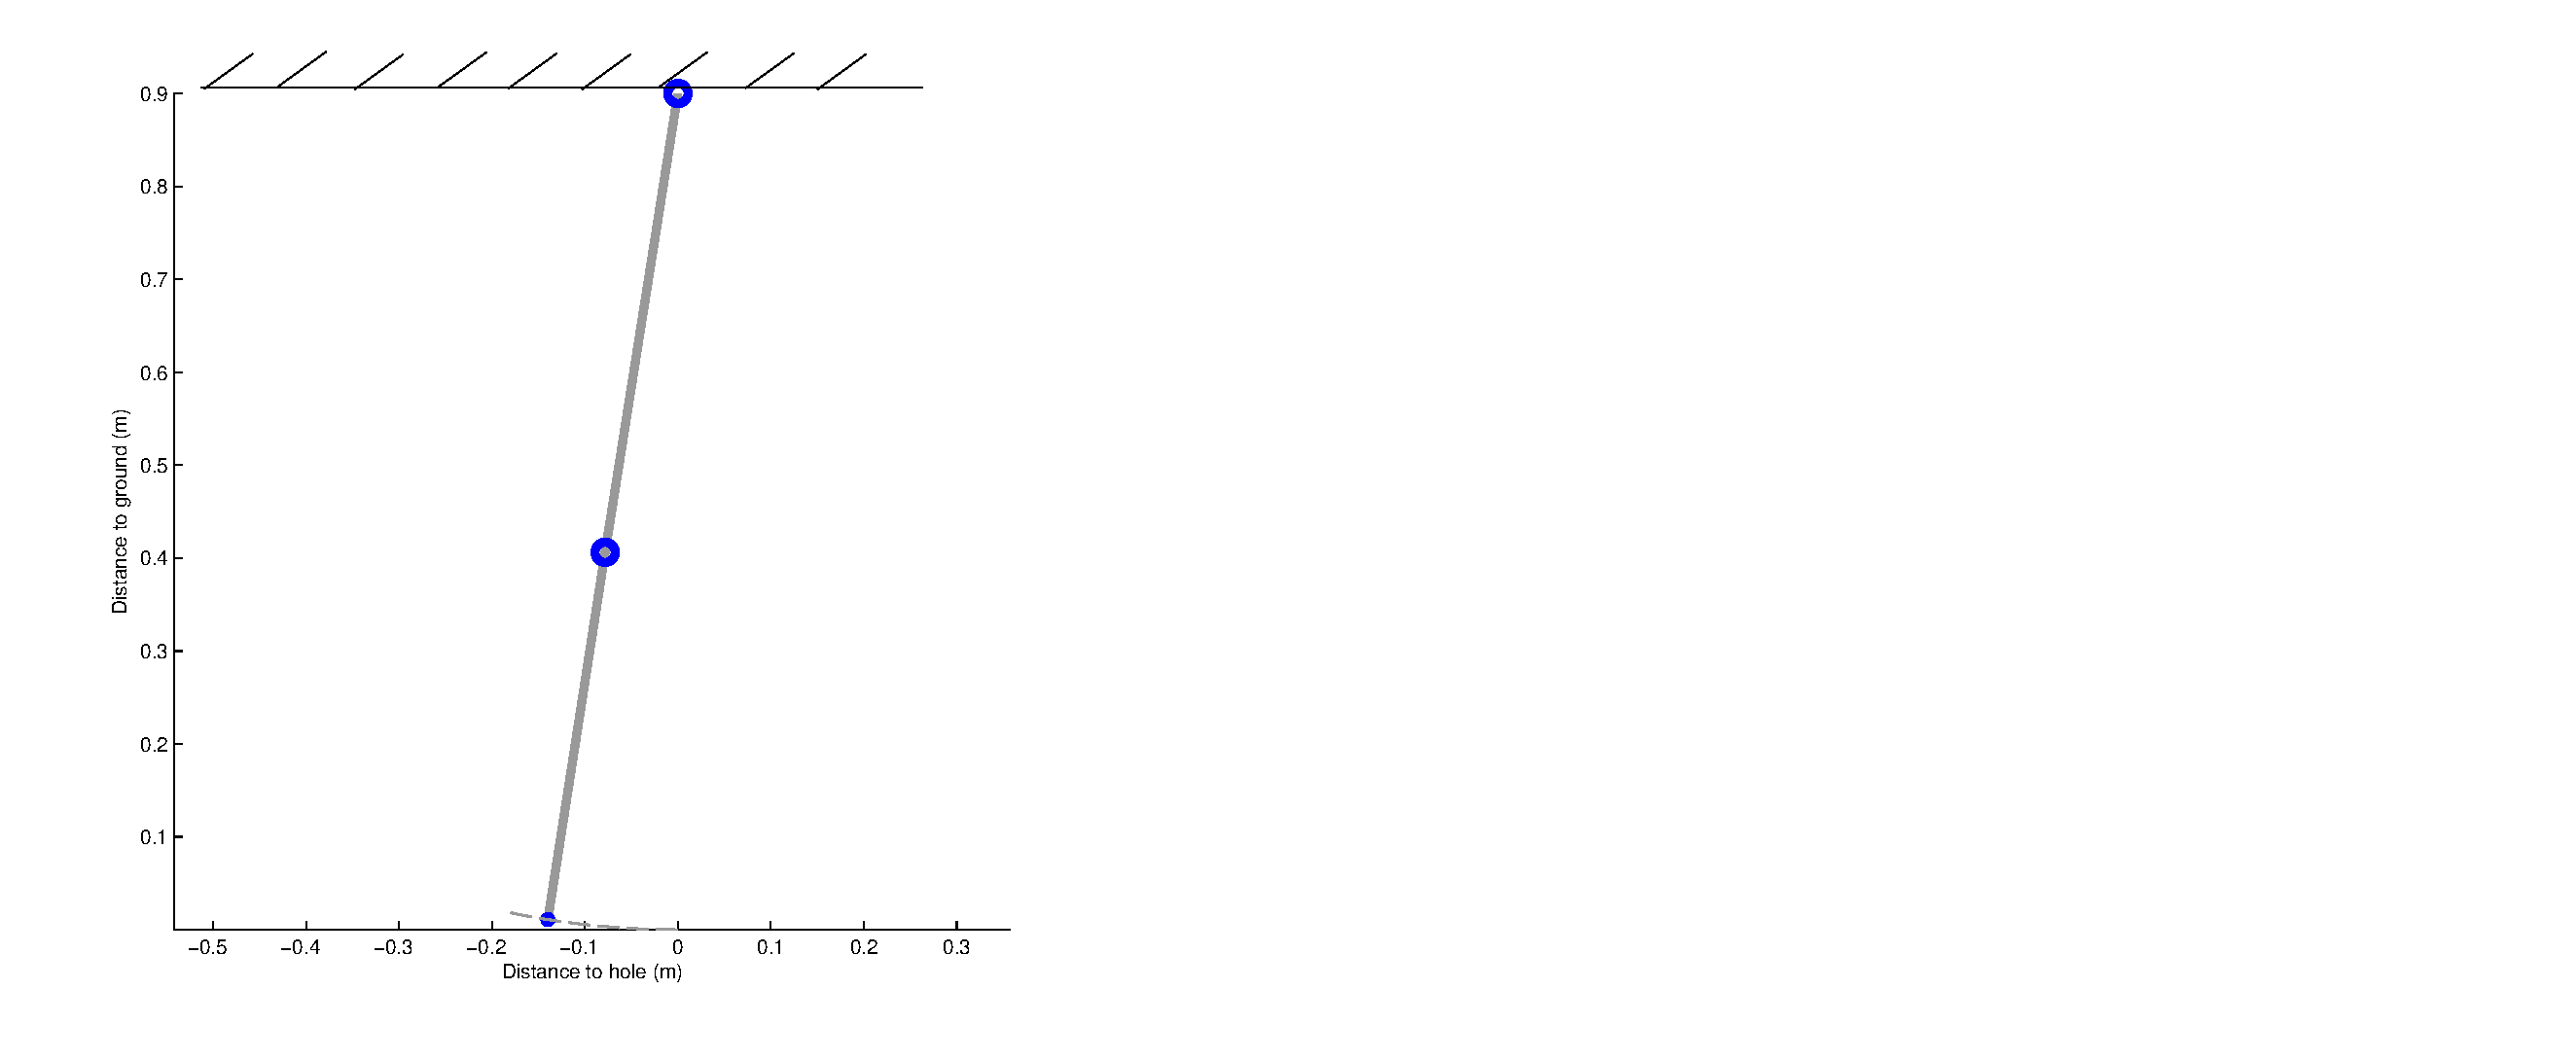
\includegraphics[width=0.5\linewidth]{putting0.eps}
\label{fig:subfig1}}
\subfloat[Final trajectory]{%
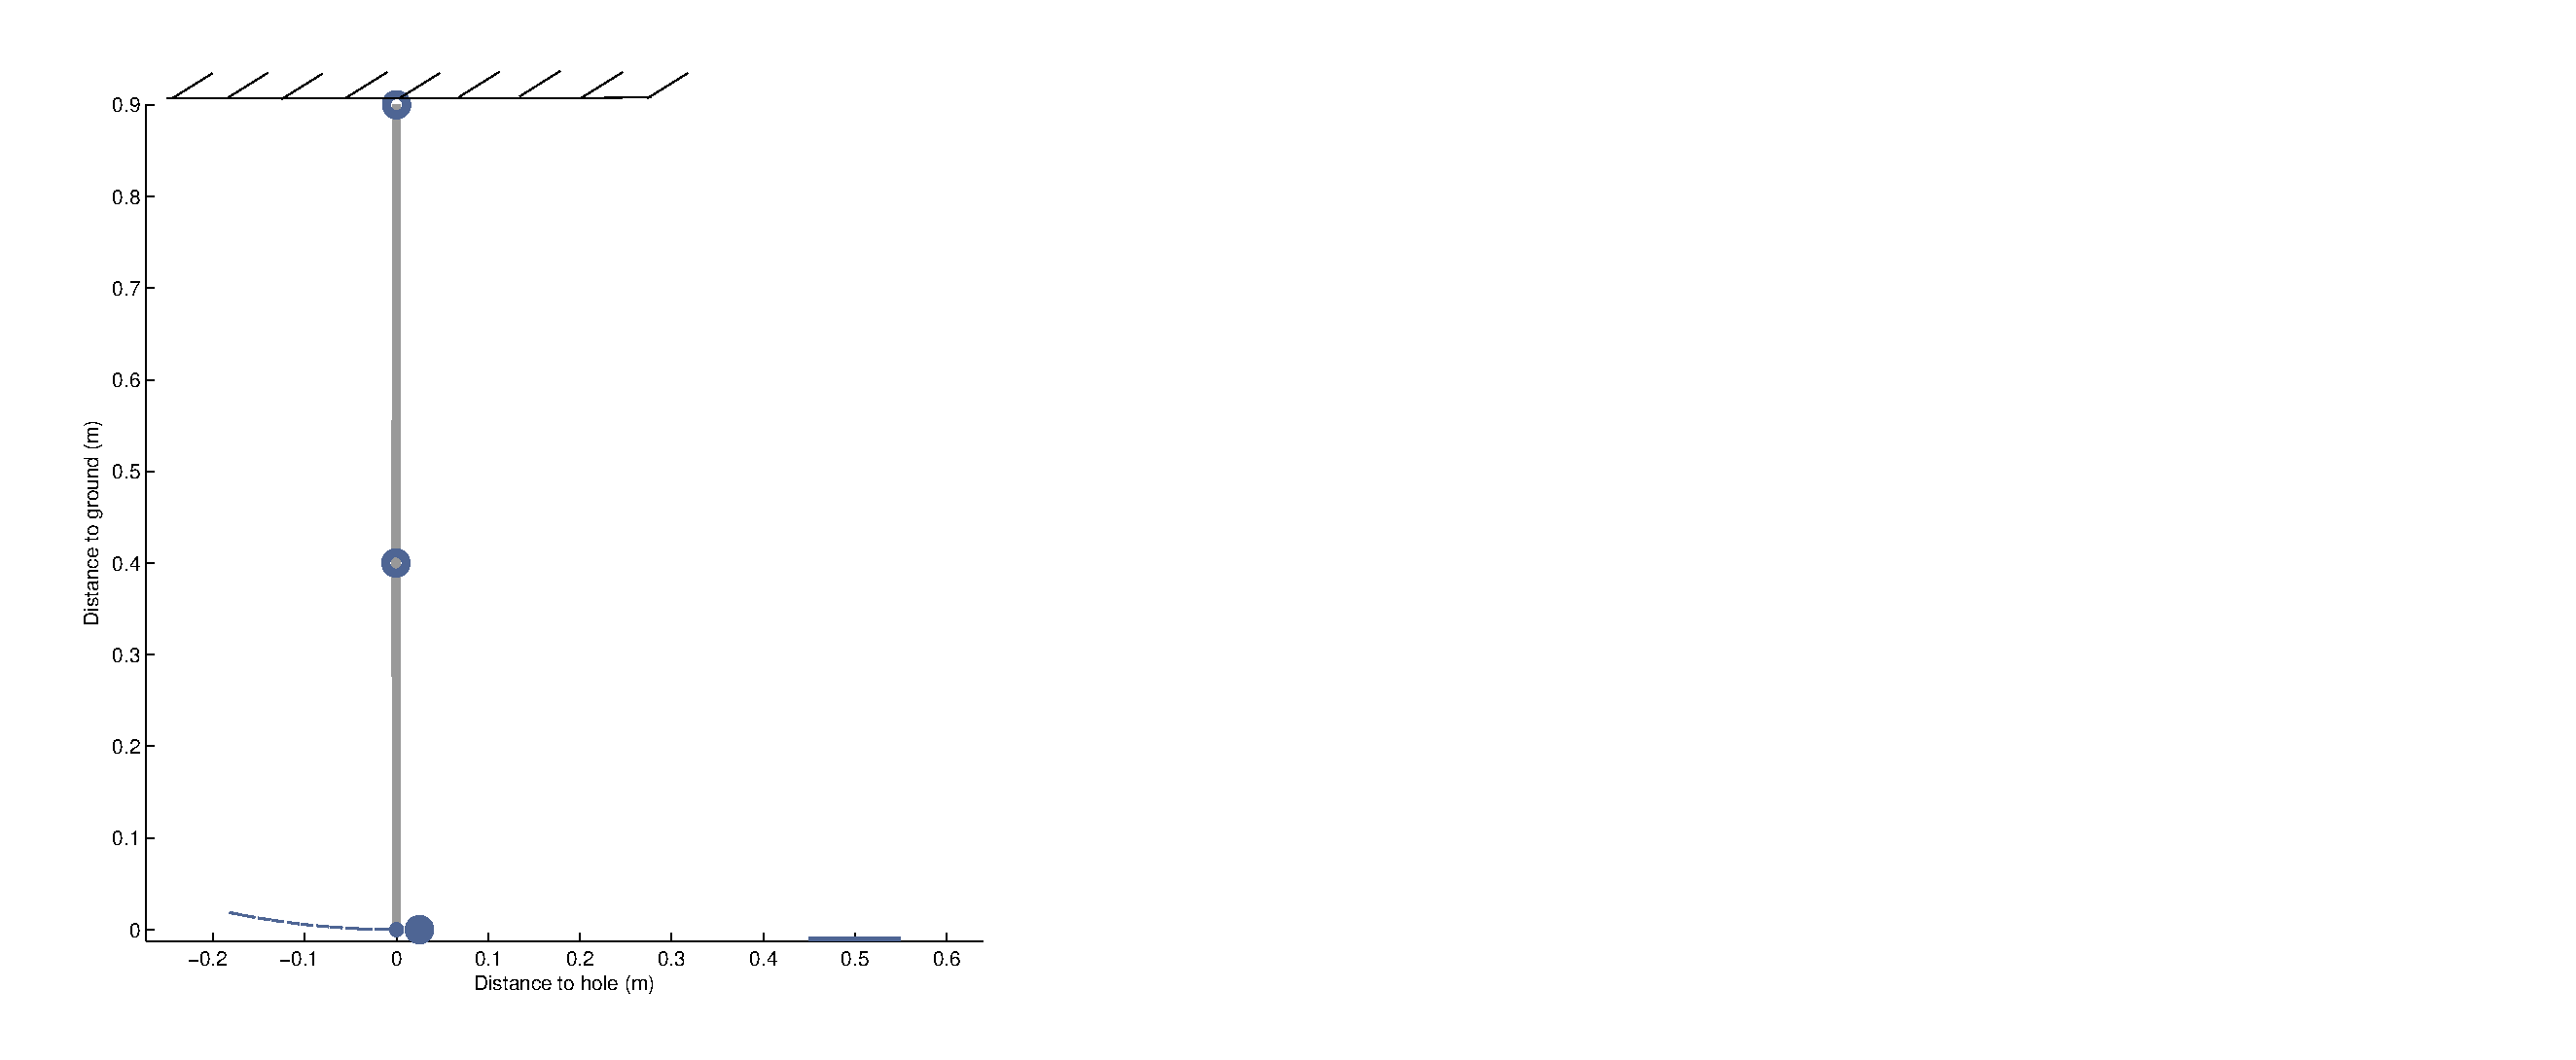
\includegraphics[width=0.5\linewidth]{putting1.eps}
\label{fig:subfig2}}
\caption{Robot arm must follow the assigned reference trajectory precisely in order to hit the ball with a desired velocity at the desired time. The reference trajectory is shown as a blue dashed curve. We can see in Fig.~\ref{fig:subfig1} that the initial attempt falls short of the reference trajectory. ILC then modifies the weights of the DMP to compensate for the modeling errors. In Fig.~\ref{fig:subfig2} the reference trajectory is executed perfectly. The ball will then approach the hole, shown as a thick blue line at a distance of 0.5 meters, with approximately zero velocity.} 
\label{putting1} 
\end{figure}

The iterations of \emph{wILC} are shown in Figure~\ref{wILCTrajectoryPutting}. Learning takes place in the joint space of the robot, since the matrix $\vec{F}_{w}$ is constructed using the nominal dynamics model \eqref{dynamics} in joint space. The full dynamics $\dynamics(\joint,\dot{\joint},\sysInput)$ involves the nonlinear effects from both links. We can see how initially the inertial disturbances of the motors prevent the end-effector from following the trajectory precisely. The following iterations show how ILC compensates for such an effect and in the last iteration the ball is given the desired velocity to reach the hole. We compare the approach with \emph{REPS} and \emph{PI$^{2}$} in Figure~\ref{wILCTrajectoryPutting} by plotting the RMS-error of the iterations with each algorithm. The error bars indicate one standard deviation within $10$ trials with different inertial mismatches. Notice that these stochastic approaches take much longer to converge.

% Compare alternative methods, gradient descent, etc.
% table shows that $R = 0$, $Q = I$ appears to be optimal in this case.

\begin{figure}
\center
%\includegraphics[scale=0.50]{comparison.eps}
\newlength\figureheight 
\newlength\figurewidth 
\setlength\figureheight{6cm}  
\setlength\figurewidth{6cm} 
\scalebox{1.0}{% This file was created by matlab2tikz.
% Minimal pgfplots version: 1.9
%
%The latest updates can be retrieved from
%  http://www.mathworks.com/matlabcentral/fileexchange/22022-matlab2tikz
%where you can also make suggestions and rate matlab2tikz.
%
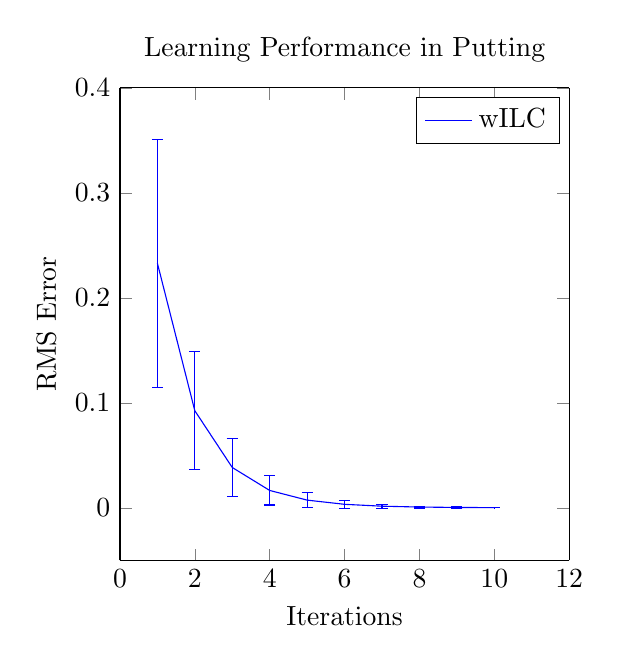
\begin{tikzpicture}

\begin{axis}[%
width=0.95092\figurewidth,
height=\figureheight,
at={(0\figurewidth,0\figureheight)},
scale only axis,
separate axis lines,
every outer x axis line/.append style={black},
every x tick label/.append style={font=\color{black}},
xmin=0,
xmax=12,
xlabel={Iterations},
every outer y axis line/.append style={black},
every y tick label/.append style={font=\color{black}},
ymin=-0.05,
ymax=0.4,
ylabel={RMS Error},
title={Learning Performance in Putting},
legend style={legend cell align=left,align=left,fill=white}
]
\addplot [color=blue,solid]
 plot [error bars/.cd, y dir = both, y explicit]
 table[row sep=crcr, y error plus index=2, y error minus index=3]{%
1	0.233032343134884	0.118115271422138	0.118115271422138\\
2	0.0924719913705091	0.0562589335711811	0.0562589335711811\\
3	0.0384258808828579	0.0276274441478736	0.0276274441478736\\
4	0.0165387503761337	0.0138614543017086	0.0138614543017086\\
5	0.00733384353006482	0.00703352539176592	0.00703352539176592\\
6	0.00333781167932676	0.00358523371207059	0.00358523371207059\\
7	0.00155369907429323	0.0018294817119812	0.0018294817119812\\
8	0.000737146368162867	0.000933121803618784	0.000933121803618784\\
9	0.000355312489801426	0.000475460765776891	0.000475460765776891\\
10	0.000173512604061655	0.000241998267982427	0.000241998267982427\\
};
\addlegendentry{wILC};

\end{axis}
\end{tikzpicture}%}
\caption{Convergence of $\alg$ to the reference putting trajectory. Convergence is quadratic for the simulated scenario where we have unknown inertial disturbances acting on the motors. Note the slow and unstable performance of the other stochastic RL algorithms.}
\label{wILCTrajectoryPutting}
\end{figure}

\subsection{Application in Table Tennis}

% hitting is not at the end of the trajectory

As a second and more complex task, we consider table tennis where we are interested in generating and executing accurate ball-hitting motions. For the robotic table tennis task we are using a seven degree of freedom (DoF) torque-controlled Barrett WAM arm capable of high speeds up to X rad/sec. A standard size racket (16 cm diameter) is mounted on the end-effector of the arm as can be seen in Figure~\ref{robot}. A vision system consisting of four cameras hanging from the ceiling around each corner of the table is used for tracking the ball \cite{Lampert12}. The orange ball is tracked  visually with a sampling rate of 60 Hz and filtered with an extended Kalman filter that accounts for some of the bouncing behavior of the ball and air drag effects. The table and the tennis balls are in accordance with the International Table Tennis Federation (ITTF) rules.

A ball launcher (see Figure~\ref{ballgun}) is available to throw balls accurately to a fixed position in Cartesian space to the forehand of the robot. The incoming ball arrives with low-variability in desired positions and higher-variability in ball velocities. The whole area to be covered amounts to about 1 m$^2$ circular region in front of the initial forehand gesture of the robot. This allows us to avoid the singularities of the robot. Any ball that appears outside of this circular \emph{feasible} region will not be hit.

When the visual system provides a trajectory of the robot that coincides with the feasible region in Cartesian space, the system has to come up with a trajectory that specifies how, where and when to intersect the incoming ball trajectory. Desired Cartesian position, velocity and orientation of the racket translates in joint space to the specification of 14 parameters: 7 joint angles and 7 joint velocities of the robot arm. Along with the desired hitting time (or the time until impact), these 15 parameters are used to train 7 joint space DMPs that corresponds to the desired reference trajectory in Cartesian space. These movement primitives are synchronized with the same phase \eqref{phase}.

% maybe work on this kinesthetic teach-in paragraph more
In order to generate feasible reference trajectories that account for the variation in incoming ball position and velocity, we used kinesthetic teach-in on the robot to generate successful hitting motions, i.e. those that can hit the ball to the opponent's court. Using the successful examples we trained a probabilistic model $p(\weights|\state_b)$ given ball positions $\state_b$ using weighted regression. Weighting can be put in various ways and we opted for a weighting which put a higher reward on the fast strikes that landed on the edges. The generated DMPs of the model are guaranteed to be safe because these movements lie within the convex combination of demonstrations. 
% Katharina - Hence, the system will not encounter joint limits or hit the table.

% scale dmps if provided with better estimation data of ball position and velocity. dmps as opposed to control inputs or even trajectories can be easily extended to allow for this. 

% From Katharina's paper:
%the position, velocity and orientation of the racket can be computed analytically based on the state of the system and the target on the opponents court.
%These task space parameters can also be converted into joint space parameters using inverse kinematics

\begin{figure}
\center
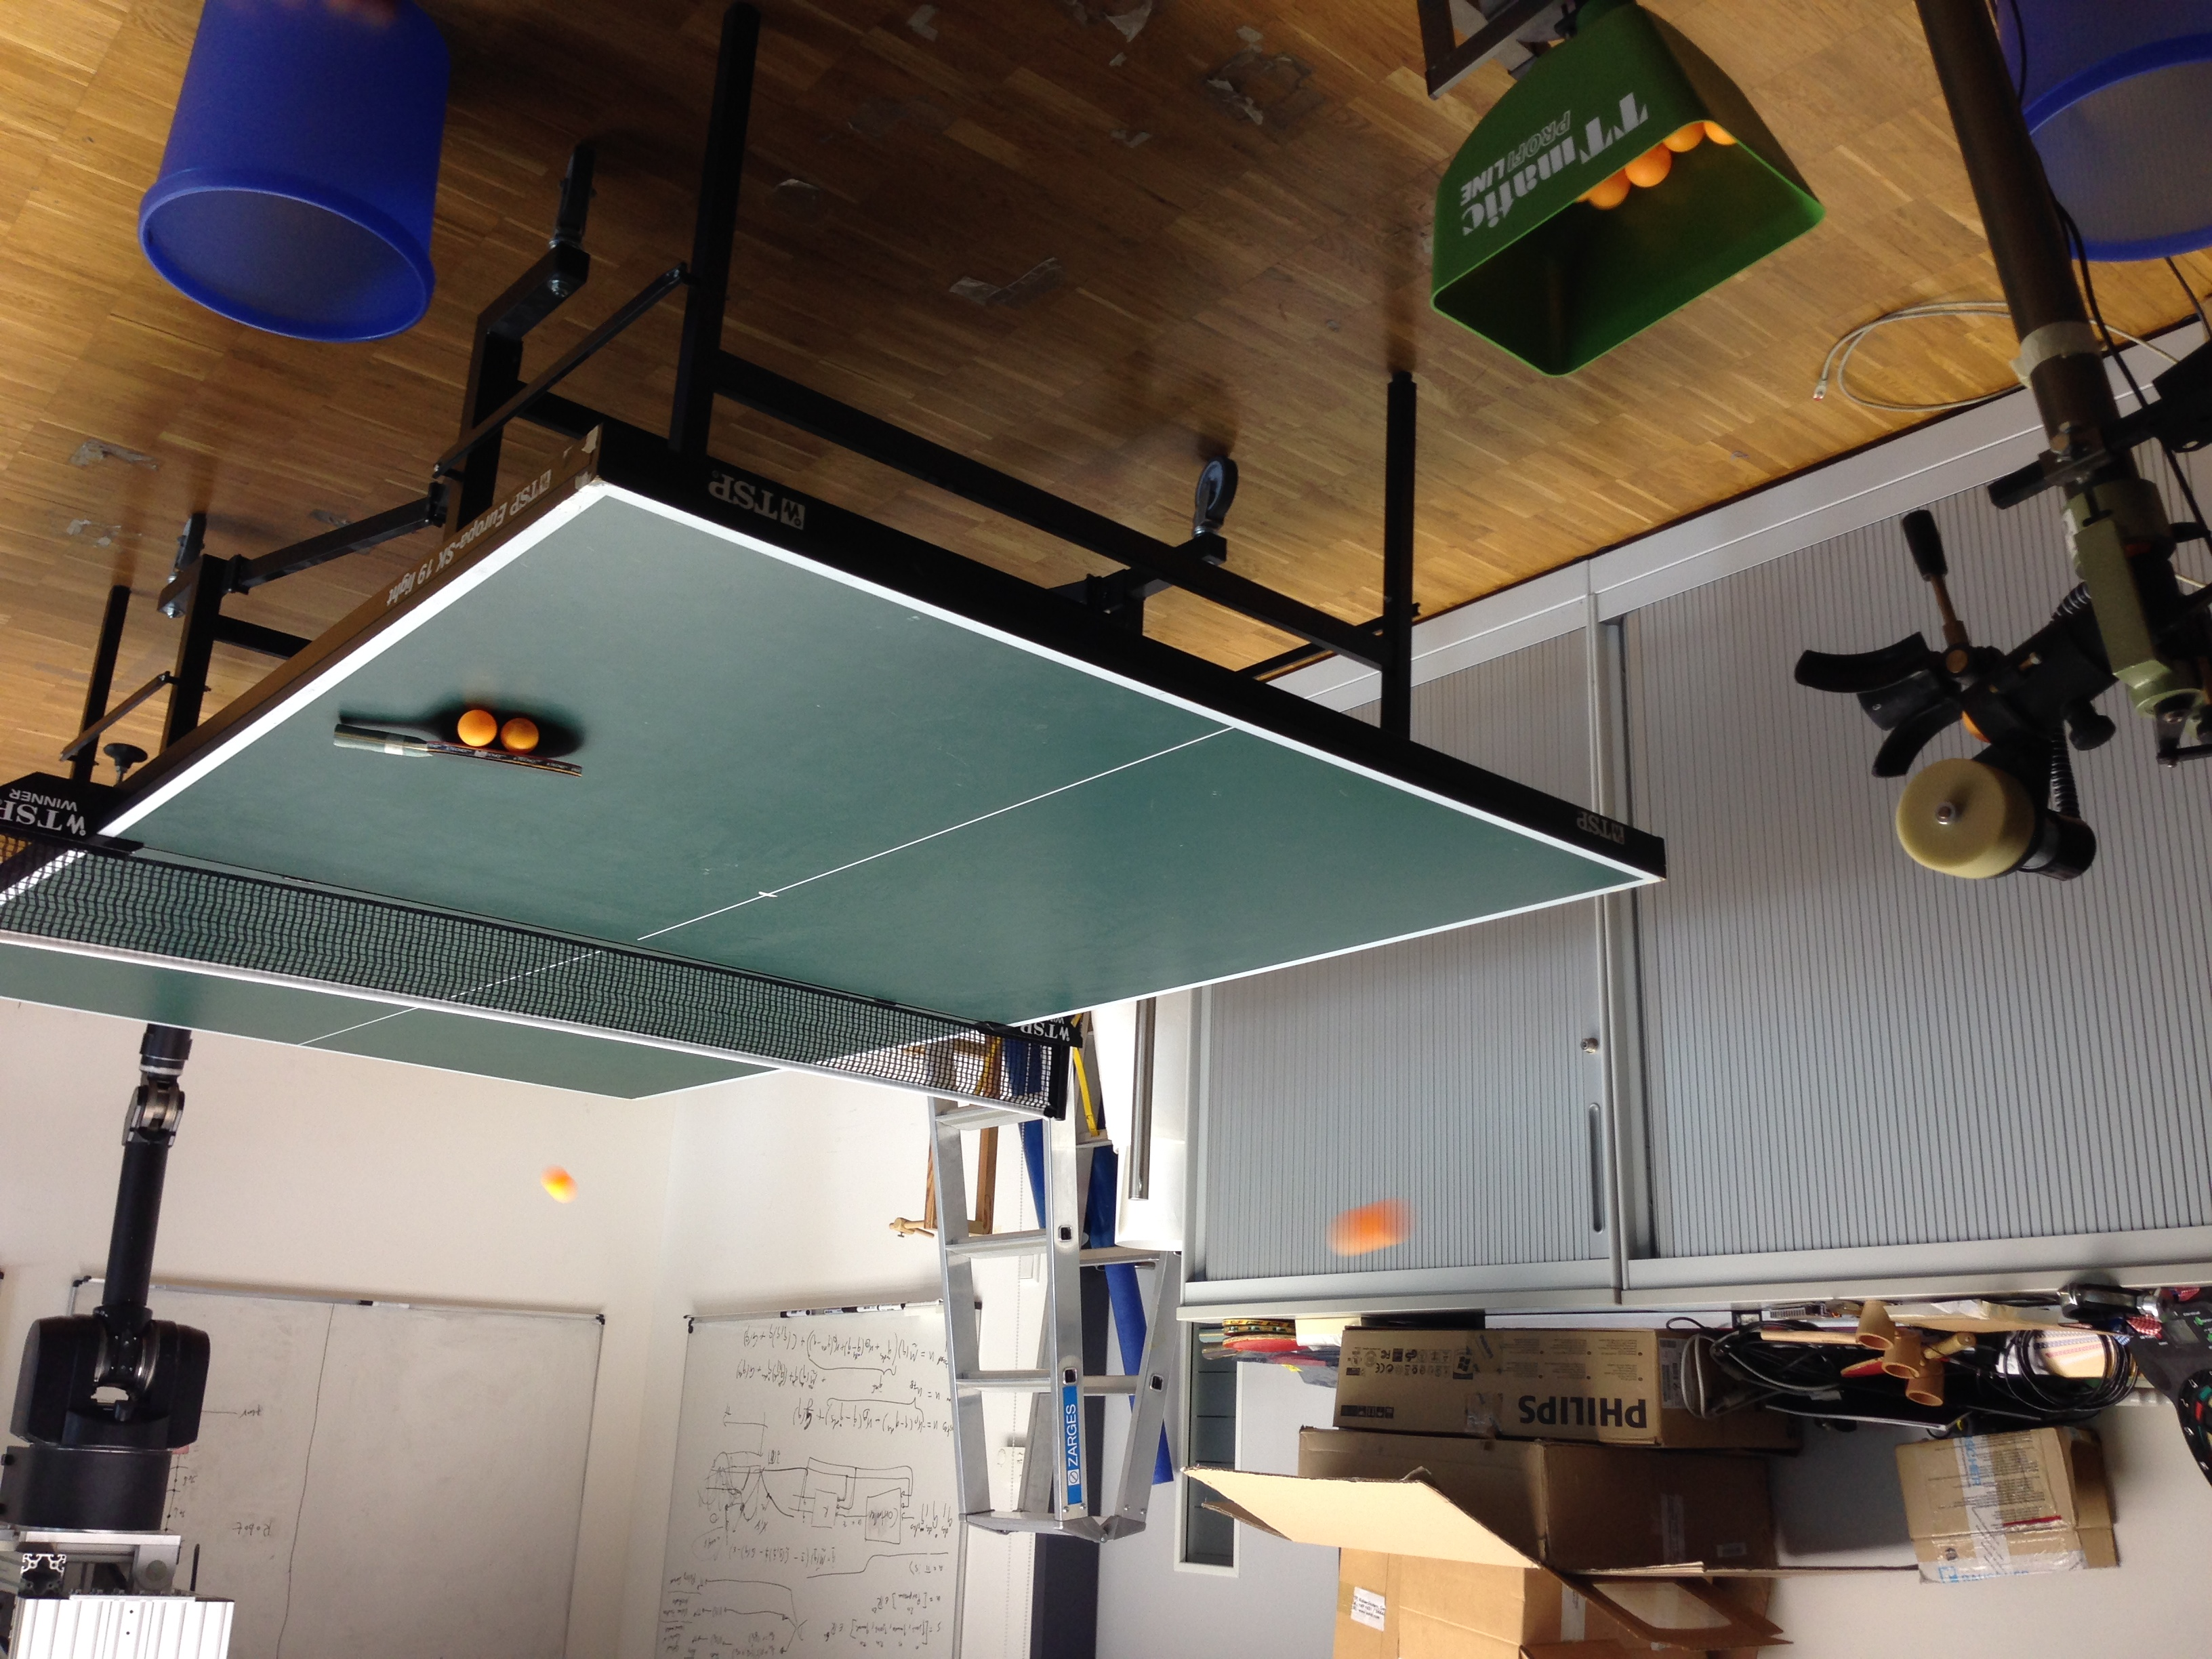
\includegraphics[scale=0.05, angle= 180]{ballgun.jpg}			
\caption{Robotic table tennis setup with the ball-launcher throwing balls to the robot}
\label{ballgun}
\end{figure}

The attached video shows the improvement achieved after using our algorithm $\alg$. In order to apply our method to a given reference trajectory, we use the mode of the empirical distribution $p(\weights,\state_b) = p(\weights|\state_b)p(\state_b)$ as the weights of our initial movement primitive. The convergence of the trajectories over the iteration domain are shown in Cartesian space in Figure~\ref{wILCTrajectoryTTCartesian}. Hard-to-model dynamical effects such as friction and stiction forces can be learned easily with our approach.

Comparisons to episodic-RL algorithms \emph{REPS} and \emph{PI$^{2}$} in Figure~\ref{ttComparison} illustrate the benefits of our approach, especially the faster convergence and increased accuracy of the proposed method. Some examples of the generated trajectories for the joints 5, 6 and 7 are given in Figure~\ref{wILCTrajectoryTT}. 

\begin{figure}
\center
%\includegraphics[scale=0.50]{comparison.eps}
\scalebox{1.0}{% This file was created by matlab2tikz v0.4.4 running on MATLAB 8.0.
% Copyright (c) 2008--2013, Nico Schlmer <nico.schloemer@gmail.com>
% All rights reserved.
% 
% The latest updates can be retrieved from
%   http://www.mathworks.com/matlabcentral/fileexchange/22022-matlab2tikz
% where you can also make suggestions and rate matlab2tikz.
% 
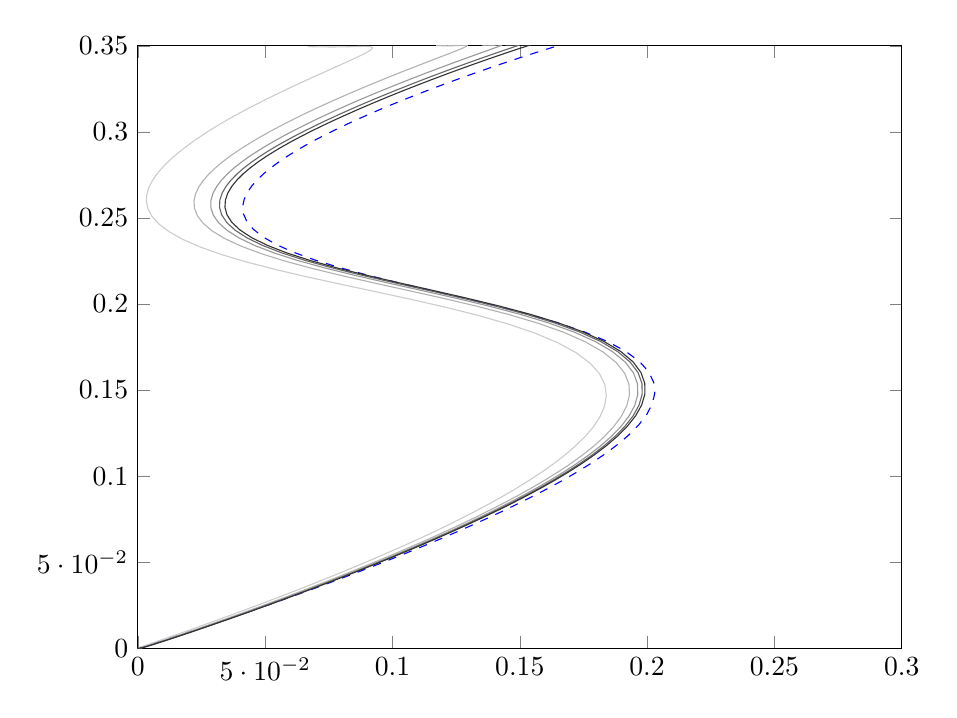
\begin{tikzpicture}

\begin{axis}[%
width=0.8\columnwidth,
height=0.630967741935484\columnwidth,
scale only axis,
xmin=0,
xmax=0.3,
ymin=0,
ymax=0.35
]
\addplot [
color=blue,
dashed,
forget plot
]
table[row sep=crcr]{
-1.22568529189217e-17 1.70219232680293e-47\\
-1.22078040529282e-17 2.17466204815869e-20\\
1.24930069097586e-15 5.59329658828069e-16\\
4.31962537102899e-13 1.9152423618868e-13\\
2.51770978879146e-11 1.11631432791867e-11\\
5.55015544523879e-10 2.46106431437956e-10\\
6.60280135771012e-09 2.9283319802688e-09\\
5.12320770129383e-08 2.27281407753508e-08\\
2.90255123674167e-07 1.28827401032052e-07\\
1.29124388293531e-06 5.73511237251698e-07\\
4.73949589296885e-06 2.10713748978966e-06\\
1.48681255318932e-05 6.6189380207418e-06\\
4.09129882041033e-05 1.82444393148059e-05\\
0.000100718153544017 4.50090857862532e-05\\
0.000225245856791989 0.000100919801590805\\
0.000463240655356511 0.000208196459707293\\
0.000884823147305501 0.000399120180670242\\
0.00158255610123486 0.000716854697447387\\
0.00266870907570527 0.00121464755420377\\
0.0042680934828865 0.00195306659807664\\
0.00650682428145541 0.00299533100932766\\
0.00949841893898853 0.00440125030957139\\
0.0133294488642299 0.00622065804358311\\
0.0180472586508033 0.00848740810159894\\
0.0236519674180277 0.0112149390444555\\
0.0300941529569334 0.0143941271208937\\
0.0372785249971626 0.0179937242124732\\
0.0450728081170337 0.0219632243456565\\
0.0533202318837492 0.0262376267222215\\
0.0618536166580361 0.0307433345872289\\
0.0705090712117028 0.0354043703208843\\
0.0791376965311413 0.0401481768418987\\
0.0876142690996799 0.0449104641836341\\
0.0958424961170963 0.0496387890730672\\
0.10375696557487 0.0542947727843779\\
0.111322280599518 0.0588550337458356\\
0.118530050316482 0.06331102120878\\
0.125394431996405 0.0676679861084513\\
0.131946828905364 0.0719433270169786\\
0.138230198729659 0.0761645191587581\\
0.144293265660084 0.0803667887860157\\
0.150184789161511 0.084590646654827\\
0.155947944238694 0.0888793518508938\\
0.161614820549927 0.0932763463165637\\
0.167201052648133 0.0978226842719481\\
0.172700648861156 0.102554481146252\\
0.178081188148765 0.107500424919056\\
0.183279696817351 0.112679429291778\\
0.188199689821794 0.11809856122523\\
0.192710046988842 0.123751440482291\\
0.196646565585241 0.12961737738435\\
0.199817148084927 0.135661573700226\\
0.202011400876493 0.141836677658674\\
0.20301387722613 0.148085506344443\\
0.202619789967853 0.154344644220661\\
0.20065273345486 0.160548886433011\\
0.196983021746862 0.166636203811203\\
0.191544736744952 0.172552738672092\\
0.184349409899893 0.178257268594913\\
0.175494381526898 0.183724581129977\\
0.165164317442443 0.188947295992029\\
0.153625080784607 0.193935846625374\\
0.1412100661361 0.198716567169214\\
0.12830006671719 0.203328087323888\\
0.115298606077758 0.207816473182085\\
0.10260527646616 0.212229725482657\\
0.0905898807700316 0.216612327368361\\
0.079570030652499 0.221000508160764\\
0.0697943393352088 0.225418764413873\\
0.0614325578259062 0.229877979341309\\
0.0545730774278078 0.234375244026284\\
0.0492273137352959 0.238895250492305\\
0.0453397371877769 0.243412935431724\\
0.0428018209176867 0.247896930561529\\
0.0414679809317703 0.252313332254143\\
0.0411716730700138 0.25662933480681\\
0.0417402386729666 0.260816396765839\\
0.0430079265640447 0.264852853167071\\
0.0448258671359753 0.268725657669276\\
0.0470681659059565 0.272431034965027\\
0.0496347242551211 0.275974250701863\\
0.0524515935766653 0.279368747748684\\
0.0554695907154709 0.282634858417776\\
0.0586617700544091 0.285798252905515\\
0.0620201947143181 0.288888235420426\\
0.0655523003124128 0.291935958228636\\
0.0692770158504934 0.294972594140621\\
0.0732207080290693 0.298027491449363\\
0.0774129544020573 0.301126332090716\\
0.0818821323091202 0.304289323201106\\
0.086650838109129 0.307529473239184\\
0.0917312255322955 0.310851034404806\\
0.0971204675308709 0.314248229434997\\
0.102796687767279 0.317704416545961\\
0.108715848493778 0.321191871765943\\
0.114810181592199 0.324672370955634\\
0.120988762173356 0.328098721508834\\
0.127140705706413 0.3314173160038\\
0.133141194808927 0.33457165455712\\
0.138860120113893 0.33750661939838\\
0.14417260737948 0.340173109510588\\
0.148970203575231 0.342532494031226\\
0.15317114157554 0.344560265930261\\
0.156728025765686 0.346248311683806\\
0.159631560364095 0.347605376663323\\
0.16190957122079 0.348655584952959\\
0.163621436389131 0.349435214610502\\
0.164848937801264 0.349988255460754\\
0.165685237911466 0.350361500346063\\
0.166223974647865 0.350599977591089\\
0.166550272189824 0.350743403168433\\
0.166734851771187 0.350824053127807\\
0.166831595215191 0.350866113799758\\
0.166878121826248 0.350886259282569\\
0.166898406741448 0.350895013534916\\
0.166906302339804 0.350898412202254\\
0.16690899217171 0.35089956776726\\
0.166909773384699 0.350899902896113\\
0.166909959992641 0.350899982867216\\
0.166909994843181 0.350899997792469\\
0.166909999566499 0.350899999814467\\
0.166909999980335 0.350899999991584\\
0.166909999999663 0.350899999999856\\
0.166909999999999 0.3509\\
0.16691 0.3509\\
0.16691 0.3509\\
};
\addplot [
color=white!80!black,
solid,
forget plot
]
table[row sep=crcr]{
-1.22568529189217e-17 1.70219232680293e-47\\
3.25274463507264e-06 8.35905362814104e-08\\
1.23717401990733e-05 6.51809556987925e-07\\
2.60782198962572e-05 2.10499070948953e-06\\
4.3092311772854e-05 4.74258914527822e-06\\
6.21318876894655e-05 8.7637958130708e-06\\
8.19125001256813e-05 1.42692959778432e-05\\
0.000101156688969535 2.12681872858731e-05\\
0.000118643983994053 2.97049649157848e-05\\
0.000133386193364771 3.95467615229986e-05\\
0.00014510004883005 5.10128278393354e-05\\
0.0001552465101183 6.5075416432896e-05\\
0.000168952051477796 8.43854757627399e-05\\
0.000198041564834851 0.000114740042164133\\
0.00026513772561189 0.000167083224948609\\
0.000408333337430968 0.000259824989119074\\
0.000685436662127054 0.000421023858453292\\
0.00117641921404975 0.000689800526123193\\
0.0019826628090404 0.0011163219128708\\
0.00322202345439749 0.00175987161326193\\
0.00501956323556232 0.00268488373870233\\
0.00749484404363355 0.0039552731473001\\
0.0107476267088559 0.00562781764097272\\
0.0148443828740994 0.00774561614639042\\
0.0198080260882525 0.0103326877885853\\
0.0256126991972536 0.0133905843814564\\
0.0321844810802911 0.0168975212907577\\
0.0394077642119747 0.0208100876679215\\
0.0471360843591468 0.0250671836813051\\
0.0552055623017432 0.0295955336269499\\
0.0634489323010695 0.0343159814489065\\
0.0717083475272989 0.0391497861089964\\
0.0798456440508612 0.0440242623581138\\
0.0877493512990643 0.0488773077339653\\
0.0953383119334656 0.0536605715857425\\
0.102562219474309 0.0583412200179673\\
0.109399655339149 0.0629024072076402\\
0.115854312001125 0.0673426650555623\\
0.121950058891251 0.0716744673315447\\
0.127725389733361 0.075922219782685\\
0.133227633162548 0.0801198897574413\\
0.138507154146251 0.0843084353295575\\
0.143611650722376 0.0885331395891004\\
0.148580574700905 0.0928409108464387\\
0.15343968194199 0.0972775796199095\\
0.158195747221979 0.101885211071146\\
0.16283155730666 0.106699458175359\\
0.16730141867135 0.111747006834142\\
0.171527575073714 0.117043208571809\\
0.175398110794516 0.122590056608926\\
0.17876709519038 0.128374731727528\\
0.181457870007442 0.13436901784707\\
0.183270418807971 0.140529933609352\\
0.183992840168584 0.1468017196852\\
0.183415811647512 0.153118883204305\\
0.181349255134415 0.159410354303193\\
0.177640391773053 0.165604747985411\\
0.172191559796912 0.171636409453042\\
0.164975852452944 0.177451555876\\
0.156048491179281 0.183013478959773\\
0.145551999572995 0.188305754446059\\
0.133713873420574 0.193332875414501\\
0.120836446899598 0.198118387394409\\
0.107279687175711 0.202701044925459\\
0.0934385122850055 0.207129644586298\\
0.0797168904764897 0.211457183163945\\
0.0665013860742654 0.215734973676006\\
0.0541368781104964 0.22000733245879\\
0.0429068577808264 0.224307382025773\\
0.033020059316166 0.22865437252083\\
0.0246043139118881 0.233052722129095\\
0.0177075894370749 0.237492749893384\\
0.0123053407655547 0.241952864909341\\
0.00831266795198405 0.246402818708713\\
0.00559943353492465 0.250807543394727\\
0.00400643982833325 0.255131090794861\\
0.00336099531970944 0.259340261583538\\
0.00349094963575494 0.263407694601951\\
0.00423632700566043 0.267314287640521\\
0.00545739698604056 0.271050520324513\\
0.00703909360281847 0.274616713655985\\
0.00889256053514898 0.278022468888926\\
0.0109545952245223 0.281285525081238\\
0.0131856580959084 0.284430233952467\\
0.0155669691751959 0.28748580297281\\
0.018097061806758 0.290484411403001\\
0.0207880223567336 0.293459265457746\\
0.0236615294186096 0.296442631788672\\
0.0267447249692657 0.29946387492171\\
0.0300659091430229 0.30254752444948\\
0.0336500541993982 0.305711411122957\\
0.0375141841333209 0.308964936070606\\
0.0416627620032532 0.312307571339502\\
0.0460833573873633 0.315727727789735\\
0.0507430103470991 0.319202160247643\\
0.0555858324175085 0.322696098963651\\
0.0605324459864692 0.326164288076076\\
0.0654818150895609 0.32955306358398\\
0.0703158276701347 0.332803506928079\\
0.0749066424601935 0.335855565592948\\
0.0791263436331281 0.338652851337519\\
0.0828579300985524 0.341147637015078\\
0.086006219944052 0.343305417717783\\
0.0885070089368458 0.345108336437797\\
0.0903329042299405 0.34655685170897\\
0.0914947162488735 0.34766926934375\\
0.0920380775007132 0.348479140774549\\
0.0920358866418595 0.349030952794802\\
0.0915779982342309 0.349374872001687\\
0.0907600654711163 0.349561458970446\\
0.0896734678021941 0.349637195188974\\
0.0883978262579761 0.349641406227386\\
0.0869968669564486 0.349604803855963\\
0.0855175674063735 0.349549511893666\\
0.0839918507219313 0.349490176744121\\
0.0824397444046635 0.349435647523352\\
0.0808729297318141 0.349390745172857\\
0.0792978877849283 0.349357781483348\\
0.0777182414268251 0.349337669415243\\
0.076136245249234 0.349330621539781\\
0.0745535944675742 0.349336526488321\\
0.0729717944868774 0.349355120123051\\
0.0713922993651467 0.349386049440274\\
0.0698165526897378 0.34942889134331\\
0.068245996566624 0.349483156689842\\
0.0666820730088789 0.349548290832413\\
};
\addplot [
color=white!70!black,
solid,
forget plot
]
table[row sep=crcr]{
-1.22568529189217e-17 1.70219232680293e-47\\
6.93129473689265e-06 9.64767466645037e-08\\
2.7053728010589e-05 7.53393712416719e-07\\
5.90241087723482e-05 2.43942373846901e-06\\
0.000101498155661405 5.51343408114195e-06\\
0.000153129376081493 1.02251741061884e-05\\
0.000212569038951388 1.67171588199604e-05\\
0.000278475522813864 2.50317808145982e-05\\
0.000349564364216304 3.51385921991254e-05\\
0.000424783594102553 4.70220206280164e-05\\
0.000503786426983947 6.09116511278121e-05\\
0.000587970596547154 7.77844535591212e-05\\
0.000682399652245789 0.000100292595867371\\
0.000798835848869633 0.000134233849753492\\
0.000959839481982006 0.000190556312586955\\
0.00120344120098727 0.000287681051323386\\
0.00158738733147519 0.000453687794298591\\
0.00219158773190882 0.000727729550523115\\
0.00311736305544096 0.00116001496346112\\
0.00448250910290361 0.00180987440428384\\
0.00641202948157397 0.00274178773012311\\
0.00902543036526304 0.00401970807708507\\
0.0124224207575113 0.00570043852896392\\
0.0166694253808309 0.00782708640457289\\
0.0217893165013838 0.0104236601922089\\
0.0277562016851992 0.0134916813674616\\
0.0344961305342789 0.0170093156475479\\
0.0418934719326902 0.0209330844092612\\
0.0498017431838193 0.025201803884487\\
0.0580570510257657 0.0297421012468949\\
0.0664921193903008 0.0344747144410509\\
0.0749490943067283 0.0393207933494284\\
0.083289807743699 0.0442075475846333\\
0.0914027883802557 0.0490727809439252\\
0.0992068821701957 0.053868067178828\\
0.106651790765752 0.0585605198516327\\
0.113716109160424 0.0631332660419391\\
0.120403549051503 0.0675848357938546\\
0.12673800451864 0.0719277239249715\\
0.132757998825081 0.0761863763987518\\
0.138510894368985 0.0803948155499262\\
0.144047093460022 0.0845940647197951\\
0.149414334532967 0.0888294783218773\\
0.154652112482077 0.0931480382373108\\
0.159786228723888 0.0975956474153343\\
0.164823505971776 0.102214439249045\\
0.169746781305514 0.107040127859175\\
0.174510413938733 0.1120994503015\\
0.179036702853095 0.11740779612371\\
0.183213790070021 0.122967179842902\\
0.186895805137288 0.128764782568114\\
0.1899061521658 0.134772362639757\\
0.192044878582981 0.1409468819141\\
0.193100147022395 0.1472324882047\\
0.19286269715242 0.153563556499437\\
0.19114250810376 0.159868847403178\\
0.187786850523484 0.166076780850869\\
0.182698103454159 0.172121506524738\\
0.175849394842952 0.177949080546467\\
0.167295979727899 0.183522700154989\\
0.157180417585707 0.188825927304757\\
0.145730241246288 0.193863312442234\\
0.133247818825882 0.198658504269697\\
0.120093144190204 0.203250378202201\\
0.106661152660102 0.207687847535028\\
0.0933558199927957 0.212024008470429\\
0.0805637088347397 0.216310250212964\\
0.0686296882127832 0.220590940806223\\
0.0578372317943576 0.224899231308802\\
0.0483950494317936 0.229254379779297\\
0.0404309416589472 0.233660794691578\\
0.0339928399182604 0.238108770890859\\
0.029056157412647 0.242576681968768\\
0.0255359478476862 0.247034235902087\\
0.0233020233782072 0.25144631659818\\
0.022195132642067 0.255776926658629\\
0.0220425280052933 0.259992820280044\\
0.0226720014664253 0.264066596454024\\
0.0239235191055781 0.267979123522436\\
0.0256572927278969 0.271720864841182\\
0.0277581997534111 0.275292139685674\\
0.0301373289229437 0.278702562031931\\
0.0327314247052732 0.281969896717172\\
0.0355008966451315 0.285118531913417\\
0.0384269160159032 0.288177719212875\\
0.0415079695590667 0.29117968640564\\
0.0447560992523834 0.294157689412887\\
0.0481929416503832 0.297144042766935\\
0.0518455992455894 0.300168154376497\\
0.0557423354994946 0.303254590408189\\
0.0599080890900244 0.306421209410366\\
0.0643598537911934 0.309677429863546\\
0.0691020660270022 0.313022729303285\\
0.0741222724777841 0.31644551101468\\
0.0793874940891376 0.319922508214131\\
0.0848418269794431 0.3234189148495\\
0.0904058815988261 0.326889423920117\\
0.0959786131876827 0.330280306170263\\
0.101441903661408 0.333532565762175\\
0.106667908232484 0.336586064933916\\
0.111528710145165 0.339384328716674\\
0.115907310598752 0.341879550643571\\
0.119708534372898 0.344037164229383\\
0.12286818970643 0.345839278347961\\
0.125358902890373 0.347286351236394\\
0.127191509935881 0.348396722962202\\
0.128411673995255 0.349204008280944\\
0.129092327454437 0.349752776234616\\
0.129323359924559 0.350093282717987\\
0.129200459903221 0.350276173935389\\
0.128815042047515 0.350348005584898\\
0.128246762583773 0.350348161750893\\
0.127559383036323 0.350307395802087\\
0.126799916704839 0.350247857240857\\
0.126000322945996 0.350184204555702\\
0.1251806659329 0.350125288184074\\
0.124352663973483 0.350075922368641\\
0.123522835457299 0.350038406444803\\
0.122694840758248 0.350013636784894\\
0.12187097212178 0.350001806250653\\
0.12105296251271 0.350002781183144\\
0.120242355145558 0.350016272815784\\
0.119440641921753 0.350041901264811\\
0.11864930428768 0.350079214324527\\
0.117869822211852 0.350127691516173\\
0.117103675565859 0.350186744625179\\
};
\addplot [
color=lightgray!80!black,
solid,
forget plot
]
table[row sep=crcr]{
-1.22568529189217e-17 1.70219232680293e-47\\
8.24119022140355e-06 1.00732406791694e-07\\
3.22818627429921e-05 7.86940656335505e-07\\
7.07559323208588e-05 2.54986090125147e-06\\
0.000122296228331723 5.76797064381405e-06\\
0.00018553338427912 1.07077012838254e-05\\
0.000259095822954879 1.75253638232066e-05\\
0.000341619118787306 2.62743262033844e-05\\
0.000431796062051802 3.69323957213372e-05\\
0.000528552011866369 4.94896975186751e-05\\
0.000631517600857057 6.41792322979517e-05\\
0.000742068082289762 8.19795699039566e-05\\
0.000865244631480491 0.000105543401475197\\
0.00101278723256497 0.000140668999415314\\
0.00120723400539919 0.000198306249405875\\
0.00148659350872234 0.000296880649727077\\
0.00190859005869599 0.000464480052181126\\
0.002553111603022 0.000740269632660934\\
0.00352145704973565 0.00117447363800878\\
0.00493140077336401 0.00182643993469807\\
0.00690792553655244 0.00276066560601727\\
0.00957051760868816 0.00404111845209194\\
0.013018867428092 0.00572461167681009\\
0.0173193828571617 0.00785425676069301\\
0.0224949212787883 0.0104540595927566\\
0.0285195774988574 0.0135255320009586\\
0.035319390500034 0.017046823099313\\
0.0427787205908372 0.0209744310901322\\
0.0507510783541073 0.0252471431363759\\
0.0590725654150967 0.0297915525019845\\
0.0675759019452456 0.0345283599239281\\
0.0761032313718057 0.0393786768622851\\
0.0845163841555275 0.0442696758156739\\
0.0927038886619868 0.0491391274533087\\
0.100584591960087 0.0539385788040041\\
0.108108198522499 0.0586351248731017\\
0.115253308079248 0.0632118832043138\\
0.122023639052197 0.0676673832532119\\
0.128443094156398 0.0720141273595286\\
0.134550207016313 0.076276575782572\\
0.140392351886249 0.0804887703534101\\
0.146019944204992 0.0846917575060123\\
0.151480736630151 0.0889309168345366\\
0.156814239248724 0.0932532561315467\\
0.162046269569075 0.0977047037845897\\
0.167183667267311 0.102327417068251\\
0.172209287258199 0.107157131409542\\
0.177077507480326 0.112220601573851\\
0.181710646551086 0.117533230120374\\
0.18599686704668 0.123097038618307\\
0.189790319960976 0.128899207779441\\
0.192914431638598 0.134911486360631\\
0.195169272283309 0.141090815579626\\
0.196343027377081 0.147381309838045\\
0.196226458744299 0.153717296801278\\
0.194629565937674 0.160027476514049\\
0.191399637271586 0.166240199323007\\
0.18643906636242 0.172289545207232\\
0.179720993560132 0.178121512882846\\
0.171300685919523 0.183699265895567\\
0.16132071575316 0.189006361231044\\
0.15000862915004 0.194047369705262\\
0.137666806389296 0.198845976718071\\
0.124655250930212 0.203441100722334\\
0.11136890434015 0.207881696624692\\
0.0982117451440555 0.212220896144709\\
0.0855703354850615 0.216510115804387\\
0.0737895409198586 0.220793742315416\\
0.0631528289654475 0.225104937212302\\
0.0538689008840692 0.229462961720491\\
0.0460655463836004 0.233872221219448\\
0.0397906840306257 0.238323002294295\\
0.0350197122887116 0.242793666223433\\
0.0316676684619934 0.247253905761631\\
0.0296043468694794 0.251668587890903\\
0.0286704771406535 0.256001697867092\\
0.0286932917590319 0.260219973468202\\
0.0295005622973088 0.264295999581883\\
0.0309322342141809 0.268210634111924\\
0.0328484988224416 0.271954334638874\\
0.0351342134438643 0.275527419817031\\
0.0377004473008033 0.278939508125996\\
0.0404839260303129 0.282208373537663\\
0.0434450410789383 0.285358417140878\\
0.0465649463701479 0.288418906155873\\
0.0498421120540551 0.291422085547991\\
0.0532885643012866 0.294401228807807\\
0.0569259246939338 0.297388667359027\\
0.060781281661924 0.300413824369689\\
0.0648828856070467 0.303501278808989\\
0.0692556632508983 0.306668898869657\\
0.0739165976105503 0.309926108924857\\
0.0788701156320308 0.313272388148497\\
0.0841037558484537 0.316696136786902\\
0.0895845324026466 0.320174080001135\\
0.0952565359222051 0.323671398441293\\
0.101040372596916 0.327142766524831\\
0.106834994514794 0.330534431396352\\
0.112522281411398 0.333787369354094\\
0.117974387199522 0.336841411957749\\
0.123063394734693 0.339640053057411\\
0.127672305965782 0.342135457664629\\
0.131705947986898 0.344293037104961\\
0.135100133412516 0.346094887844805\\
0.137827495291969 0.3475414677501\\
0.139898878703717 0.348651128804713\\
0.141359957684072 0.349457508011248\\
0.142283676615549 0.350005203379756\\
0.142759937586791 0.350344502272953\\
0.142884441669828 0.350526081058766\\
0.142748616062309 0.350596521548441\\
0.14243212952282 0.350595228378737\\
0.141998756175451 0.350552969484934\\
0.141495522047665 0.350491903311688\\
0.140954399376044 0.350426692491499\\
0.140395465359062 0.350366187815311\\
0.13983045145243 0.350315201062375\\
0.139265889288576 0.350276027090483\\
0.138705452554353 0.350249556355617\\
0.138151446857674 0.350235974722749\\
0.137605618559151 0.350235140647284\\
0.13706952429002 0.350246756673952\\
0.136544669380156 0.350270433458172\\
0.136032548709625 0.350305708569233\\
0.135534655681571 0.350352050539719\\
0.135052483600492 0.350408859401613\\
};
\addplot [
color=gray!80!black,
solid,
forget plot
]
table[row sep=crcr]{
-1.22568529189217e-17 1.70219232680293e-47\\
8.92977877512262e-06 1.02875256139306e-07\\
3.50302073670603e-05 8.03832204998465e-07\\
7.6923181451443e-05 2.6054666526772e-06\\
0.000133229513849615 5.89612735388159e-06\\
0.000202567829414407 1.09506412435071e-05\\
0.000283554556587495 1.79322606298721e-05\\
0.000374813297083546 2.68998738572252e-05\\
0.000475024898264518 3.78354390567461e-05\\
0.00058310281472824 5.07319460217592e-05\\
0.000698665821066556 6.58241162764799e-05\\
0.000823077365168913 8.40913381849907e-05\\
0.000961366872516901 0.000108186603085048\\
0.00112526263206191 0.000143908514171362\\
0.0013372911192877 0.000202208001417812\\
0.00163544929455634 0.000301513027909894\\
0.00207744991934694 0.000469915878014372\\
0.00274316943818554 0.00074658831036123\\
0.00373389534015586 0.0011817629856139\\
0.00516739074226722 0.00183479720468099\\
0.00716862744585325 0.00277019737138397\\
0.00985708124108685 0.00405193928677507\\
0.0133324327779902 0.00573684179051188\\
0.017661081015106 0.00786801888227079\\
0.0228658754619511 0.0104694754201866\\
0.0289209041629876 0.0135427184867887\\
0.0357522004656874 0.0170658887717894\\
0.0432441201229809 0.0209954725658302\\
0.0512501701454335 0.0252702419822597\\
0.0596064494404405 0.0298167726496399\\
0.0681456761811332 0.0345557458973301\\
0.0767099924117116 0.0394082531059054\\
0.0851612277883653 0.0443014473555745\\
0.0933879105000287 0.0491730819721281\\
0.101308888187009 0.0539746899928377\\
0.108873866784702 0.0586733567120258\\
0.116061448486722 0.0632521946938633\\
0.122875355216972 0.0677097331068654\\
0.12933949419109 0.0720584782550339\\
0.135492404436783 0.0763228979085512\\
0.141381466394777 0.0805370441269593\\
0.147057102358845 0.0847419754453117\\
0.152567072418053 0.0889830846373902\\
0.157950894604189 0.0933073930400802\\
0.163234394848169 0.0977608423175764\\
0.168424421712857 0.102385602185229\\
0.173503839465477 0.10721741914209\\
0.178427035872348 0.11228305712342\\
0.183116339864578 0.11759792538159\\
0.187459924821671 0.123164049044482\\
0.191311953014686 0.128968608470596\\
0.194495862483409 0.134983347244226\\
0.196811735414456 0.141165195614265\\
0.198047769311679 0.147458250317859\\
0.197994737657609 0.153796814064669\\
0.196462650751454 0.160109555005934\\
0.193298806206009 0.166324786867196\\
0.188405605310313 0.172376552959401\\
0.18175619494662 0.178210821802491\\
0.173405848500447 0.183790739213434\\
0.163497145047472 0.189099859549082\\
0.152257637664544 0.194142764317839\\
0.139989713044845 0.19894315820053\\
0.12705337971325 0.203539982274023\\
0.113843582544761 0.207982213333711\\
0.100764301543973 0.212323001802113\\
0.0882020986142179 0.216613778612594\\
0.0765018375125098 0.220898940359292\\
0.0659469825469476 0.22521165416738\\
0.0567462304884415 0.229571183020556\\
0.049027365378689 0.233981930769087\\
0.0428382990414638 0.238434179751384\\
0.0381544222191173 0.242906284861195\\
0.0348907636219798 0.247367930928288\\
0.0329171082219877 0.251783976100636\\
0.0320741756852476 0.256118396564673\\
0.0321891880715997 0.260337921502582\\
0.0330899062427278 0.264415128410756\\
0.0346162648409108 0.2683308697187\\
0.036628444427112 0.272075599975723\\
0.0390112917748274 0.275649637507928\\
0.0416758658592514 0.279062603155282\\
0.0445588824278458 0.282332275679604\\
0.0476207234201685 0.285483062942925\\
0.0508425336436436 0.288544240358539\\
0.0542227745293641 0.291548061892158\\
0.0577734639401573 0.294527810235089\\
0.0615162155887227 0.29751582564768\\
0.0654781105140704 0.300541539268275\\
0.069687392254882 0.303629536735988\\
0.0741689812505039 0.306797691244088\\
0.0789398548670954 0.310055430185055\\
0.0840044350727047 0.31340223350734\\
0.0893502561221372 0.316826499765939\\
0.0949443285860845 0.320304949788047\\
0.10073074020827 0.323802757130865\\
0.106630094939127 0.327274586340627\\
0.112541343206658 0.330666672055047\\
0.118346363594059 0.333919975828261\\
0.123917309320733 0.336974313002536\\
0.129126263024408 0.339773160953013\\
0.133856227032223 0.342268669620473\\
0.138012029638276 0.344426238592833\\
0.141529485741297 0.346227957742641\\
0.144381231929687 0.347674284668092\\
0.146578118038222 0.348783577541131\\
0.148165823818506 0.349589484978445\\
0.149217299956915 0.350136620133057\\
0.14982245510157 0.350475286822565\\
0.15007699693636 0.350656177185017\\
0.150072359252929 0.350725886677099\\
0.149888217398158 0.350723830665718\\
0.149588352117699 0.350680784680134\\
0.149219796125307 0.350618911814269\\
0.148814528421328 0.350552876839747\\
0.14839263304238 0.350491530705835\\
0.147965848345104 0.350439683880285\\
0.147540712911789 0.350399628860669\\
0.147120907415342 0.350372252995834\\
0.146708744475372 0.350357738484599\\
0.146305977481483 0.35035593965763\\
0.145914170104769 0.350366554521367\\
0.145534834721014 0.350389188795593\\
0.145169473258873 0.350423374720786\\
0.1448195861705 0.35046857510784\\
0.144486673808429 0.350524183873566\\
};
\addplot [
color=darkgray!80!black,
solid,
forget plot
]
table[row sep=crcr]{
-1.22568529189217e-17 1.70219232680293e-47\\
9.3599787039213e-06 1.0417101912332e-07\\
3.67472565733727e-05 8.14046240397971e-07\\
8.07762283287326e-05 2.63908981594335e-06\\
0.000140060207390276 5.97361816027719e-06\\
0.000213210324072626 1.10975329272605e-05\\
0.000298835521074842 1.81782813127163e-05\\
0.000395551927675744 2.72780870527299e-05\\
0.000502032937133339 3.83814155625667e-05\\
0.000617184573577938 5.14829869834302e-05\\
0.00074061820980064 6.68185639616807e-05\\
0.000873689924463659 8.5368036054316e-05\\
0.00102142180835642 0.000109784593732231\\
0.00119553484998007 0.000145867077780254\\
0.00141854825650836 0.000204567118240015\\
0.00172845174930132 0.000304314279952965\\
0.0021829508785694 0.000473203690687496\\
0.00286191490956714 0.000750411307059446\\
0.00386662420340855 0.0011861751429198\\
0.00531483484716441 0.00183985850187608\\
0.00733151179290929 0.00277597373183081\\
0.0100361242771989 0.00405850176585805\\
0.0135283468221219 0.00574426510863267\\
0.0178745728054188 0.00787637948475917\\
0.0230976467956264 0.0104788492611891\\
0.0291716525890287 0.0135531787042616\\
0.0360226199889105 0.0170775033788272\\
0.043534901880865 0.021008302256862\\
0.051562003026155 0.0252843381546641\\
0.0599400206208809 0.0298321757695653\\
0.0685016715802959 0.0345724843748974\\
0.0770890970779875 0.0394263428602883\\
0.0855641262624378 0.0443208922158884\\
0.0938152872071621 0.0491938749645788\\
0.101761427903042 0.0539968154279506\\
0.109352255190543 0.0586967928535431\\
0.116566372790718 0.0632769167100027\\
0.123407504800645 0.067735715997117\\
0.129899561230249 0.0720856995007324\\
0.136081084463359 0.0763513396822957\\
0.141999458784845 0.0805666949831835\\
0.147705110750004 0.0847728314821394\\
0.153245805070229 0.0890151501618397\\
0.158661064721878 0.0933406807870793\\
0.163976720881216 0.0977953732740882\\
0.169199627649344 0.102421405060018\\
0.174312655125908 0.107254529503681\\
0.179270197209958 0.112321516206356\\
0.183994589272221 0.117637778535721\\
0.188374011440659 0.123205343775658\\
0.192262633033297 0.129011391998196\\
0.195483899399841 0.135027663494474\\
0.197837900217713 0.141211081605555\\
0.199112840506493 0.147505731986089\\
0.199099501037313 0.153845901717464\\
0.197607898828365 0.160160238997701\\
0.194485337306686 0.166377034653828\\
0.18963422255999 0.172430309075094\\
0.183027705557095 0.178266011906733\\
0.174721063644686 0.183847277881476\\
0.164856880130506 0.189157659706088\\
0.153662712464837 0.19420174556224\\
0.141440951356884 0.199003252172211\\
0.128551608506045 0.20360113474741\\
0.115389630864249 0.208044383764832\\
0.102358999371317 0.212386161346023\\
0.0898462757916453 0.216677907450459\\
0.0781963227686839 0.220964024876747\\
0.0676926026164741 0.225277684279662\\
0.0585438093107243 0.2296381497825\\
0.0508777233642002 0.234049824323025\\
0.0447422523995665 0.238502987628501\\
0.040112782347364 0.24297599064265\\
0.0369043365614955 0.247438513277933\\
0.0349866941872291 0.251855408191103\\
0.0342005686790319 0.256190645923996\\
0.0343731755972173 0.260410950304008\\
0.0353322691237018 0.264488894219923\\
0.0369177771540226 0.268405326686834\\
0.0389898735413398 0.272150700362392\\
0.0414333984769443 0.275725333366954\\
0.0441594045403562 0.279138848012056\\
0.0471046013052596 0.282409026046797\\
0.0502293647751702 0.28556027955736\\
0.053514834064677 0.288621889065871\\
0.0569594651593455 0.291626114148557\\
0.0605752707329631 0.294606243229344\\
0.0643838595829539 0.297594622070293\\
0.0684123081321 0.300620686766432\\
0.0726888556329081 0.3037090270971\\
0.0772384186018462 0.306877519348699\\
0.0820779708770266 0.310135592764979\\
0.0872119313191577 0.313482727739413\\
0.0926278315128938 0.316907321728181\\
0.0982926797997083 0.320386092806208\\
0.104150562123465 0.32388421005322\\
0.110122081036359 0.327356331801865\\
0.116106185928705 0.330748684830497\\
0.121984754661522 0.334002221438116\\
0.12762994001709 0.337056746794087\\
0.132913824491634 0.339855727942772\\
0.137719410642107 0.342351305374223\\
0.141951527505355 0.344508871310043\\
0.145545991400554 0.346310511470982\\
0.148475441121506 0.347756683255383\\
0.150750729470393 0.348865748667293\\
0.152417539767093 0.349671363543548\\
0.153548826635592 0.350218150460284\\
0.154234502822518 0.350556423476957\\
0.154570280143574 0.350736884546155\\
0.154647596510981 0.350806137613783\\
0.154546131387969 0.350803604718214\\
0.154329669656292 0.35076006610554\\
0.154045248205047 0.350697687752151\\
0.153724850257181 0.350631135749437\\
0.153388564117416 0.350569261134261\\
0.153048132449003 0.350516873548681\\
0.152710098170926 0.350476264014004\\
0.15237814631509 0.350448317940478\\
0.152054593875948 0.350433215243187\\
0.151741198628649 0.350430807686562\\
0.151439528636546 0.350440790456397\\
0.151151100671428 0.350462766207533\\
0.150877421059584 0.350496263873815\\
0.150619994651039 0.350540742717994\\
0.150380326195567 0.350595592866864\\
};
\end{axis}
\end{tikzpicture}%}
\caption{Convergence of $\alg$ to the reference table tennis trajectory in Cartesian space.}
\label{wILCTrajectoryTTCartesian}
\end{figure}

\begin{figure}
\center
%\includegraphics[scale=0.50]{comparison.eps}
\scalebox{1.0}{% This file was created by matlab2tikz v0.4.4 running on MATLAB 8.0.
% Copyright (c) 2008--2013, Nico Schlmer <nico.schloemer@gmail.com>
% All rights reserved.
% 
% The latest updates can be retrieved from
%   http://www.mathworks.com/matlabcentral/fileexchange/22022-matlab2tikz
% where you can also make suggestions and rate matlab2tikz.
% 
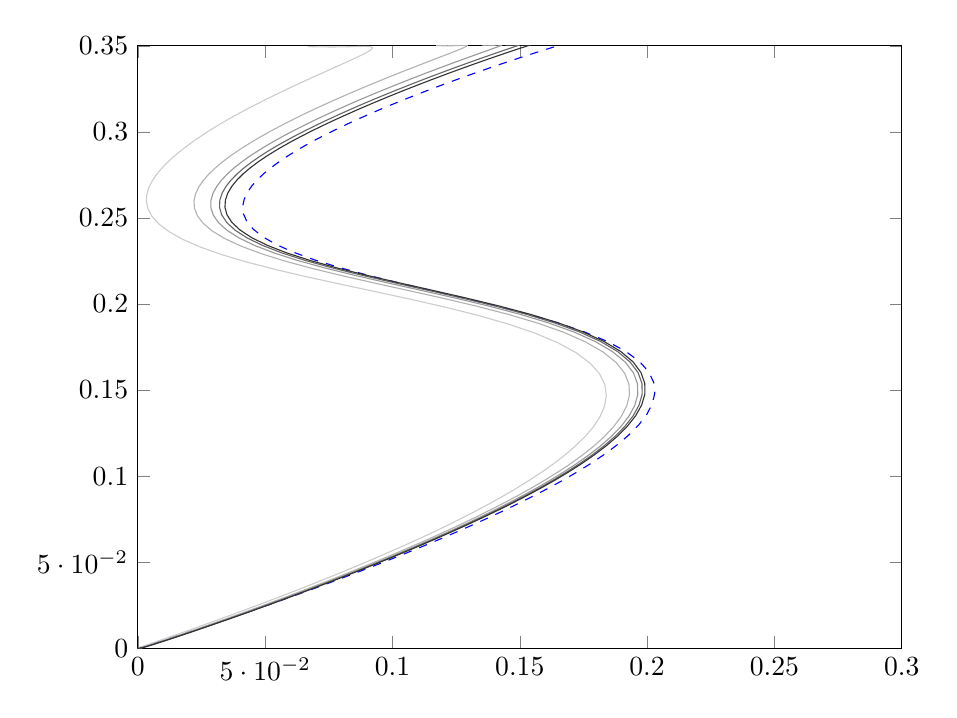
\begin{tikzpicture}

\begin{axis}[%
width=0.8\columnwidth,
height=0.630967741935484\columnwidth,
scale only axis,
xmin=0,
xmax=0.3,
ymin=0,
ymax=0.35
]
\addplot [
color=blue,
dashed,
forget plot
]
table[row sep=crcr]{
-1.22568529189217e-17 1.70219232680293e-47\\
-1.22078040529282e-17 2.17466204815869e-20\\
1.24930069097586e-15 5.59329658828069e-16\\
4.31962537102899e-13 1.9152423618868e-13\\
2.51770978879146e-11 1.11631432791867e-11\\
5.55015544523879e-10 2.46106431437956e-10\\
6.60280135771012e-09 2.9283319802688e-09\\
5.12320770129383e-08 2.27281407753508e-08\\
2.90255123674167e-07 1.28827401032052e-07\\
1.29124388293531e-06 5.73511237251698e-07\\
4.73949589296885e-06 2.10713748978966e-06\\
1.48681255318932e-05 6.6189380207418e-06\\
4.09129882041033e-05 1.82444393148059e-05\\
0.000100718153544017 4.50090857862532e-05\\
0.000225245856791989 0.000100919801590805\\
0.000463240655356511 0.000208196459707293\\
0.000884823147305501 0.000399120180670242\\
0.00158255610123486 0.000716854697447387\\
0.00266870907570527 0.00121464755420377\\
0.0042680934828865 0.00195306659807664\\
0.00650682428145541 0.00299533100932766\\
0.00949841893898853 0.00440125030957139\\
0.0133294488642299 0.00622065804358311\\
0.0180472586508033 0.00848740810159894\\
0.0236519674180277 0.0112149390444555\\
0.0300941529569334 0.0143941271208937\\
0.0372785249971626 0.0179937242124732\\
0.0450728081170337 0.0219632243456565\\
0.0533202318837492 0.0262376267222215\\
0.0618536166580361 0.0307433345872289\\
0.0705090712117028 0.0354043703208843\\
0.0791376965311413 0.0401481768418987\\
0.0876142690996799 0.0449104641836341\\
0.0958424961170963 0.0496387890730672\\
0.10375696557487 0.0542947727843779\\
0.111322280599518 0.0588550337458356\\
0.118530050316482 0.06331102120878\\
0.125394431996405 0.0676679861084513\\
0.131946828905364 0.0719433270169786\\
0.138230198729659 0.0761645191587581\\
0.144293265660084 0.0803667887860157\\
0.150184789161511 0.084590646654827\\
0.155947944238694 0.0888793518508938\\
0.161614820549927 0.0932763463165637\\
0.167201052648133 0.0978226842719481\\
0.172700648861156 0.102554481146252\\
0.178081188148765 0.107500424919056\\
0.183279696817351 0.112679429291778\\
0.188199689821794 0.11809856122523\\
0.192710046988842 0.123751440482291\\
0.196646565585241 0.12961737738435\\
0.199817148084927 0.135661573700226\\
0.202011400876493 0.141836677658674\\
0.20301387722613 0.148085506344443\\
0.202619789967853 0.154344644220661\\
0.20065273345486 0.160548886433011\\
0.196983021746862 0.166636203811203\\
0.191544736744952 0.172552738672092\\
0.184349409899893 0.178257268594913\\
0.175494381526898 0.183724581129977\\
0.165164317442443 0.188947295992029\\
0.153625080784607 0.193935846625374\\
0.1412100661361 0.198716567169214\\
0.12830006671719 0.203328087323888\\
0.115298606077758 0.207816473182085\\
0.10260527646616 0.212229725482657\\
0.0905898807700316 0.216612327368361\\
0.079570030652499 0.221000508160764\\
0.0697943393352088 0.225418764413873\\
0.0614325578259062 0.229877979341309\\
0.0545730774278078 0.234375244026284\\
0.0492273137352959 0.238895250492305\\
0.0453397371877769 0.243412935431724\\
0.0428018209176867 0.247896930561529\\
0.0414679809317703 0.252313332254143\\
0.0411716730700138 0.25662933480681\\
0.0417402386729666 0.260816396765839\\
0.0430079265640447 0.264852853167071\\
0.0448258671359753 0.268725657669276\\
0.0470681659059565 0.272431034965027\\
0.0496347242551211 0.275974250701863\\
0.0524515935766653 0.279368747748684\\
0.0554695907154709 0.282634858417776\\
0.0586617700544091 0.285798252905515\\
0.0620201947143181 0.288888235420426\\
0.0655523003124128 0.291935958228636\\
0.0692770158504934 0.294972594140621\\
0.0732207080290693 0.298027491449363\\
0.0774129544020573 0.301126332090716\\
0.0818821323091202 0.304289323201106\\
0.086650838109129 0.307529473239184\\
0.0917312255322955 0.310851034404806\\
0.0971204675308709 0.314248229434997\\
0.102796687767279 0.317704416545961\\
0.108715848493778 0.321191871765943\\
0.114810181592199 0.324672370955634\\
0.120988762173356 0.328098721508834\\
0.127140705706413 0.3314173160038\\
0.133141194808927 0.33457165455712\\
0.138860120113893 0.33750661939838\\
0.14417260737948 0.340173109510588\\
0.148970203575231 0.342532494031226\\
0.15317114157554 0.344560265930261\\
0.156728025765686 0.346248311683806\\
0.159631560364095 0.347605376663323\\
0.16190957122079 0.348655584952959\\
0.163621436389131 0.349435214610502\\
0.164848937801264 0.349988255460754\\
0.165685237911466 0.350361500346063\\
0.166223974647865 0.350599977591089\\
0.166550272189824 0.350743403168433\\
0.166734851771187 0.350824053127807\\
0.166831595215191 0.350866113799758\\
0.166878121826248 0.350886259282569\\
0.166898406741448 0.350895013534916\\
0.166906302339804 0.350898412202254\\
0.16690899217171 0.35089956776726\\
0.166909773384699 0.350899902896113\\
0.166909959992641 0.350899982867216\\
0.166909994843181 0.350899997792469\\
0.166909999566499 0.350899999814467\\
0.166909999980335 0.350899999991584\\
0.166909999999663 0.350899999999856\\
0.166909999999999 0.3509\\
0.16691 0.3509\\
0.16691 0.3509\\
};
\addplot [
color=white!80!black,
solid,
forget plot
]
table[row sep=crcr]{
-1.22568529189217e-17 1.70219232680293e-47\\
3.25274463507264e-06 8.35905362814104e-08\\
1.23717401990733e-05 6.51809556987925e-07\\
2.60782198962572e-05 2.10499070948953e-06\\
4.3092311772854e-05 4.74258914527822e-06\\
6.21318876894655e-05 8.7637958130708e-06\\
8.19125001256813e-05 1.42692959778432e-05\\
0.000101156688969535 2.12681872858731e-05\\
0.000118643983994053 2.97049649157848e-05\\
0.000133386193364771 3.95467615229986e-05\\
0.00014510004883005 5.10128278393354e-05\\
0.0001552465101183 6.5075416432896e-05\\
0.000168952051477796 8.43854757627399e-05\\
0.000198041564834851 0.000114740042164133\\
0.00026513772561189 0.000167083224948609\\
0.000408333337430968 0.000259824989119074\\
0.000685436662127054 0.000421023858453292\\
0.00117641921404975 0.000689800526123193\\
0.0019826628090404 0.0011163219128708\\
0.00322202345439749 0.00175987161326193\\
0.00501956323556232 0.00268488373870233\\
0.00749484404363355 0.0039552731473001\\
0.0107476267088559 0.00562781764097272\\
0.0148443828740994 0.00774561614639042\\
0.0198080260882525 0.0103326877885853\\
0.0256126991972536 0.0133905843814564\\
0.0321844810802911 0.0168975212907577\\
0.0394077642119747 0.0208100876679215\\
0.0471360843591468 0.0250671836813051\\
0.0552055623017432 0.0295955336269499\\
0.0634489323010695 0.0343159814489065\\
0.0717083475272989 0.0391497861089964\\
0.0798456440508612 0.0440242623581138\\
0.0877493512990643 0.0488773077339653\\
0.0953383119334656 0.0536605715857425\\
0.102562219474309 0.0583412200179673\\
0.109399655339149 0.0629024072076402\\
0.115854312001125 0.0673426650555623\\
0.121950058891251 0.0716744673315447\\
0.127725389733361 0.075922219782685\\
0.133227633162548 0.0801198897574413\\
0.138507154146251 0.0843084353295575\\
0.143611650722376 0.0885331395891004\\
0.148580574700905 0.0928409108464387\\
0.15343968194199 0.0972775796199095\\
0.158195747221979 0.101885211071146\\
0.16283155730666 0.106699458175359\\
0.16730141867135 0.111747006834142\\
0.171527575073714 0.117043208571809\\
0.175398110794516 0.122590056608926\\
0.17876709519038 0.128374731727528\\
0.181457870007442 0.13436901784707\\
0.183270418807971 0.140529933609352\\
0.183992840168584 0.1468017196852\\
0.183415811647512 0.153118883204305\\
0.181349255134415 0.159410354303193\\
0.177640391773053 0.165604747985411\\
0.172191559796912 0.171636409453042\\
0.164975852452944 0.177451555876\\
0.156048491179281 0.183013478959773\\
0.145551999572995 0.188305754446059\\
0.133713873420574 0.193332875414501\\
0.120836446899598 0.198118387394409\\
0.107279687175711 0.202701044925459\\
0.0934385122850055 0.207129644586298\\
0.0797168904764897 0.211457183163945\\
0.0665013860742654 0.215734973676006\\
0.0541368781104964 0.22000733245879\\
0.0429068577808264 0.224307382025773\\
0.033020059316166 0.22865437252083\\
0.0246043139118881 0.233052722129095\\
0.0177075894370749 0.237492749893384\\
0.0123053407655547 0.241952864909341\\
0.00831266795198405 0.246402818708713\\
0.00559943353492465 0.250807543394727\\
0.00400643982833325 0.255131090794861\\
0.00336099531970944 0.259340261583538\\
0.00349094963575494 0.263407694601951\\
0.00423632700566043 0.267314287640521\\
0.00545739698604056 0.271050520324513\\
0.00703909360281847 0.274616713655985\\
0.00889256053514898 0.278022468888926\\
0.0109545952245223 0.281285525081238\\
0.0131856580959084 0.284430233952467\\
0.0155669691751959 0.28748580297281\\
0.018097061806758 0.290484411403001\\
0.0207880223567336 0.293459265457746\\
0.0236615294186096 0.296442631788672\\
0.0267447249692657 0.29946387492171\\
0.0300659091430229 0.30254752444948\\
0.0336500541993982 0.305711411122957\\
0.0375141841333209 0.308964936070606\\
0.0416627620032532 0.312307571339502\\
0.0460833573873633 0.315727727789735\\
0.0507430103470991 0.319202160247643\\
0.0555858324175085 0.322696098963651\\
0.0605324459864692 0.326164288076076\\
0.0654818150895609 0.32955306358398\\
0.0703158276701347 0.332803506928079\\
0.0749066424601935 0.335855565592948\\
0.0791263436331281 0.338652851337519\\
0.0828579300985524 0.341147637015078\\
0.086006219944052 0.343305417717783\\
0.0885070089368458 0.345108336437797\\
0.0903329042299405 0.34655685170897\\
0.0914947162488735 0.34766926934375\\
0.0920380775007132 0.348479140774549\\
0.0920358866418595 0.349030952794802\\
0.0915779982342309 0.349374872001687\\
0.0907600654711163 0.349561458970446\\
0.0896734678021941 0.349637195188974\\
0.0883978262579761 0.349641406227386\\
0.0869968669564486 0.349604803855963\\
0.0855175674063735 0.349549511893666\\
0.0839918507219313 0.349490176744121\\
0.0824397444046635 0.349435647523352\\
0.0808729297318141 0.349390745172857\\
0.0792978877849283 0.349357781483348\\
0.0777182414268251 0.349337669415243\\
0.076136245249234 0.349330621539781\\
0.0745535944675742 0.349336526488321\\
0.0729717944868774 0.349355120123051\\
0.0713922993651467 0.349386049440274\\
0.0698165526897378 0.34942889134331\\
0.068245996566624 0.349483156689842\\
0.0666820730088789 0.349548290832413\\
};
\addplot [
color=white!70!black,
solid,
forget plot
]
table[row sep=crcr]{
-1.22568529189217e-17 1.70219232680293e-47\\
6.93129473689265e-06 9.64767466645037e-08\\
2.7053728010589e-05 7.53393712416719e-07\\
5.90241087723482e-05 2.43942373846901e-06\\
0.000101498155661405 5.51343408114195e-06\\
0.000153129376081493 1.02251741061884e-05\\
0.000212569038951388 1.67171588199604e-05\\
0.000278475522813864 2.50317808145982e-05\\
0.000349564364216304 3.51385921991254e-05\\
0.000424783594102553 4.70220206280164e-05\\
0.000503786426983947 6.09116511278121e-05\\
0.000587970596547154 7.77844535591212e-05\\
0.000682399652245789 0.000100292595867371\\
0.000798835848869633 0.000134233849753492\\
0.000959839481982006 0.000190556312586955\\
0.00120344120098727 0.000287681051323386\\
0.00158738733147519 0.000453687794298591\\
0.00219158773190882 0.000727729550523115\\
0.00311736305544096 0.00116001496346112\\
0.00448250910290361 0.00180987440428384\\
0.00641202948157397 0.00274178773012311\\
0.00902543036526304 0.00401970807708507\\
0.0124224207575113 0.00570043852896392\\
0.0166694253808309 0.00782708640457289\\
0.0217893165013838 0.0104236601922089\\
0.0277562016851992 0.0134916813674616\\
0.0344961305342789 0.0170093156475479\\
0.0418934719326902 0.0209330844092612\\
0.0498017431838193 0.025201803884487\\
0.0580570510257657 0.0297421012468949\\
0.0664921193903008 0.0344747144410509\\
0.0749490943067283 0.0393207933494284\\
0.083289807743699 0.0442075475846333\\
0.0914027883802557 0.0490727809439252\\
0.0992068821701957 0.053868067178828\\
0.106651790765752 0.0585605198516327\\
0.113716109160424 0.0631332660419391\\
0.120403549051503 0.0675848357938546\\
0.12673800451864 0.0719277239249715\\
0.132757998825081 0.0761863763987518\\
0.138510894368985 0.0803948155499262\\
0.144047093460022 0.0845940647197951\\
0.149414334532967 0.0888294783218773\\
0.154652112482077 0.0931480382373108\\
0.159786228723888 0.0975956474153343\\
0.164823505971776 0.102214439249045\\
0.169746781305514 0.107040127859175\\
0.174510413938733 0.1120994503015\\
0.179036702853095 0.11740779612371\\
0.183213790070021 0.122967179842902\\
0.186895805137288 0.128764782568114\\
0.1899061521658 0.134772362639757\\
0.192044878582981 0.1409468819141\\
0.193100147022395 0.1472324882047\\
0.19286269715242 0.153563556499437\\
0.19114250810376 0.159868847403178\\
0.187786850523484 0.166076780850869\\
0.182698103454159 0.172121506524738\\
0.175849394842952 0.177949080546467\\
0.167295979727899 0.183522700154989\\
0.157180417585707 0.188825927304757\\
0.145730241246288 0.193863312442234\\
0.133247818825882 0.198658504269697\\
0.120093144190204 0.203250378202201\\
0.106661152660102 0.207687847535028\\
0.0933558199927957 0.212024008470429\\
0.0805637088347397 0.216310250212964\\
0.0686296882127832 0.220590940806223\\
0.0578372317943576 0.224899231308802\\
0.0483950494317936 0.229254379779297\\
0.0404309416589472 0.233660794691578\\
0.0339928399182604 0.238108770890859\\
0.029056157412647 0.242576681968768\\
0.0255359478476862 0.247034235902087\\
0.0233020233782072 0.25144631659818\\
0.022195132642067 0.255776926658629\\
0.0220425280052933 0.259992820280044\\
0.0226720014664253 0.264066596454024\\
0.0239235191055781 0.267979123522436\\
0.0256572927278969 0.271720864841182\\
0.0277581997534111 0.275292139685674\\
0.0301373289229437 0.278702562031931\\
0.0327314247052732 0.281969896717172\\
0.0355008966451315 0.285118531913417\\
0.0384269160159032 0.288177719212875\\
0.0415079695590667 0.29117968640564\\
0.0447560992523834 0.294157689412887\\
0.0481929416503832 0.297144042766935\\
0.0518455992455894 0.300168154376497\\
0.0557423354994946 0.303254590408189\\
0.0599080890900244 0.306421209410366\\
0.0643598537911934 0.309677429863546\\
0.0691020660270022 0.313022729303285\\
0.0741222724777841 0.31644551101468\\
0.0793874940891376 0.319922508214131\\
0.0848418269794431 0.3234189148495\\
0.0904058815988261 0.326889423920117\\
0.0959786131876827 0.330280306170263\\
0.101441903661408 0.333532565762175\\
0.106667908232484 0.336586064933916\\
0.111528710145165 0.339384328716674\\
0.115907310598752 0.341879550643571\\
0.119708534372898 0.344037164229383\\
0.12286818970643 0.345839278347961\\
0.125358902890373 0.347286351236394\\
0.127191509935881 0.348396722962202\\
0.128411673995255 0.349204008280944\\
0.129092327454437 0.349752776234616\\
0.129323359924559 0.350093282717987\\
0.129200459903221 0.350276173935389\\
0.128815042047515 0.350348005584898\\
0.128246762583773 0.350348161750893\\
0.127559383036323 0.350307395802087\\
0.126799916704839 0.350247857240857\\
0.126000322945996 0.350184204555702\\
0.1251806659329 0.350125288184074\\
0.124352663973483 0.350075922368641\\
0.123522835457299 0.350038406444803\\
0.122694840758248 0.350013636784894\\
0.12187097212178 0.350001806250653\\
0.12105296251271 0.350002781183144\\
0.120242355145558 0.350016272815784\\
0.119440641921753 0.350041901264811\\
0.11864930428768 0.350079214324527\\
0.117869822211852 0.350127691516173\\
0.117103675565859 0.350186744625179\\
};
\addplot [
color=lightgray!80!black,
solid,
forget plot
]
table[row sep=crcr]{
-1.22568529189217e-17 1.70219232680293e-47\\
8.24119022140355e-06 1.00732406791694e-07\\
3.22818627429921e-05 7.86940656335505e-07\\
7.07559323208588e-05 2.54986090125147e-06\\
0.000122296228331723 5.76797064381405e-06\\
0.00018553338427912 1.07077012838254e-05\\
0.000259095822954879 1.75253638232066e-05\\
0.000341619118787306 2.62743262033844e-05\\
0.000431796062051802 3.69323957213372e-05\\
0.000528552011866369 4.94896975186751e-05\\
0.000631517600857057 6.41792322979517e-05\\
0.000742068082289762 8.19795699039566e-05\\
0.000865244631480491 0.000105543401475197\\
0.00101278723256497 0.000140668999415314\\
0.00120723400539919 0.000198306249405875\\
0.00148659350872234 0.000296880649727077\\
0.00190859005869599 0.000464480052181126\\
0.002553111603022 0.000740269632660934\\
0.00352145704973565 0.00117447363800878\\
0.00493140077336401 0.00182643993469807\\
0.00690792553655244 0.00276066560601727\\
0.00957051760868816 0.00404111845209194\\
0.013018867428092 0.00572461167681009\\
0.0173193828571617 0.00785425676069301\\
0.0224949212787883 0.0104540595927566\\
0.0285195774988574 0.0135255320009586\\
0.035319390500034 0.017046823099313\\
0.0427787205908372 0.0209744310901322\\
0.0507510783541073 0.0252471431363759\\
0.0590725654150967 0.0297915525019845\\
0.0675759019452456 0.0345283599239281\\
0.0761032313718057 0.0393786768622851\\
0.0845163841555275 0.0442696758156739\\
0.0927038886619868 0.0491391274533087\\
0.100584591960087 0.0539385788040041\\
0.108108198522499 0.0586351248731017\\
0.115253308079248 0.0632118832043138\\
0.122023639052197 0.0676673832532119\\
0.128443094156398 0.0720141273595286\\
0.134550207016313 0.076276575782572\\
0.140392351886249 0.0804887703534101\\
0.146019944204992 0.0846917575060123\\
0.151480736630151 0.0889309168345366\\
0.156814239248724 0.0932532561315467\\
0.162046269569075 0.0977047037845897\\
0.167183667267311 0.102327417068251\\
0.172209287258199 0.107157131409542\\
0.177077507480326 0.112220601573851\\
0.181710646551086 0.117533230120374\\
0.18599686704668 0.123097038618307\\
0.189790319960976 0.128899207779441\\
0.192914431638598 0.134911486360631\\
0.195169272283309 0.141090815579626\\
0.196343027377081 0.147381309838045\\
0.196226458744299 0.153717296801278\\
0.194629565937674 0.160027476514049\\
0.191399637271586 0.166240199323007\\
0.18643906636242 0.172289545207232\\
0.179720993560132 0.178121512882846\\
0.171300685919523 0.183699265895567\\
0.16132071575316 0.189006361231044\\
0.15000862915004 0.194047369705262\\
0.137666806389296 0.198845976718071\\
0.124655250930212 0.203441100722334\\
0.11136890434015 0.207881696624692\\
0.0982117451440555 0.212220896144709\\
0.0855703354850615 0.216510115804387\\
0.0737895409198586 0.220793742315416\\
0.0631528289654475 0.225104937212302\\
0.0538689008840692 0.229462961720491\\
0.0460655463836004 0.233872221219448\\
0.0397906840306257 0.238323002294295\\
0.0350197122887116 0.242793666223433\\
0.0316676684619934 0.247253905761631\\
0.0296043468694794 0.251668587890903\\
0.0286704771406535 0.256001697867092\\
0.0286932917590319 0.260219973468202\\
0.0295005622973088 0.264295999581883\\
0.0309322342141809 0.268210634111924\\
0.0328484988224416 0.271954334638874\\
0.0351342134438643 0.275527419817031\\
0.0377004473008033 0.278939508125996\\
0.0404839260303129 0.282208373537663\\
0.0434450410789383 0.285358417140878\\
0.0465649463701479 0.288418906155873\\
0.0498421120540551 0.291422085547991\\
0.0532885643012866 0.294401228807807\\
0.0569259246939338 0.297388667359027\\
0.060781281661924 0.300413824369689\\
0.0648828856070467 0.303501278808989\\
0.0692556632508983 0.306668898869657\\
0.0739165976105503 0.309926108924857\\
0.0788701156320308 0.313272388148497\\
0.0841037558484537 0.316696136786902\\
0.0895845324026466 0.320174080001135\\
0.0952565359222051 0.323671398441293\\
0.101040372596916 0.327142766524831\\
0.106834994514794 0.330534431396352\\
0.112522281411398 0.333787369354094\\
0.117974387199522 0.336841411957749\\
0.123063394734693 0.339640053057411\\
0.127672305965782 0.342135457664629\\
0.131705947986898 0.344293037104961\\
0.135100133412516 0.346094887844805\\
0.137827495291969 0.3475414677501\\
0.139898878703717 0.348651128804713\\
0.141359957684072 0.349457508011248\\
0.142283676615549 0.350005203379756\\
0.142759937586791 0.350344502272953\\
0.142884441669828 0.350526081058766\\
0.142748616062309 0.350596521548441\\
0.14243212952282 0.350595228378737\\
0.141998756175451 0.350552969484934\\
0.141495522047665 0.350491903311688\\
0.140954399376044 0.350426692491499\\
0.140395465359062 0.350366187815311\\
0.13983045145243 0.350315201062375\\
0.139265889288576 0.350276027090483\\
0.138705452554353 0.350249556355617\\
0.138151446857674 0.350235974722749\\
0.137605618559151 0.350235140647284\\
0.13706952429002 0.350246756673952\\
0.136544669380156 0.350270433458172\\
0.136032548709625 0.350305708569233\\
0.135534655681571 0.350352050539719\\
0.135052483600492 0.350408859401613\\
};
\addplot [
color=gray!80!black,
solid,
forget plot
]
table[row sep=crcr]{
-1.22568529189217e-17 1.70219232680293e-47\\
8.92977877512262e-06 1.02875256139306e-07\\
3.50302073670603e-05 8.03832204998465e-07\\
7.6923181451443e-05 2.6054666526772e-06\\
0.000133229513849615 5.89612735388159e-06\\
0.000202567829414407 1.09506412435071e-05\\
0.000283554556587495 1.79322606298721e-05\\
0.000374813297083546 2.68998738572252e-05\\
0.000475024898264518 3.78354390567461e-05\\
0.00058310281472824 5.07319460217592e-05\\
0.000698665821066556 6.58241162764799e-05\\
0.000823077365168913 8.40913381849907e-05\\
0.000961366872516901 0.000108186603085048\\
0.00112526263206191 0.000143908514171362\\
0.0013372911192877 0.000202208001417812\\
0.00163544929455634 0.000301513027909894\\
0.00207744991934694 0.000469915878014372\\
0.00274316943818554 0.00074658831036123\\
0.00373389534015586 0.0011817629856139\\
0.00516739074226722 0.00183479720468099\\
0.00716862744585325 0.00277019737138397\\
0.00985708124108685 0.00405193928677507\\
0.0133324327779902 0.00573684179051188\\
0.017661081015106 0.00786801888227079\\
0.0228658754619511 0.0104694754201866\\
0.0289209041629876 0.0135427184867887\\
0.0357522004656874 0.0170658887717894\\
0.0432441201229809 0.0209954725658302\\
0.0512501701454335 0.0252702419822597\\
0.0596064494404405 0.0298167726496399\\
0.0681456761811332 0.0345557458973301\\
0.0767099924117116 0.0394082531059054\\
0.0851612277883653 0.0443014473555745\\
0.0933879105000287 0.0491730819721281\\
0.101308888187009 0.0539746899928377\\
0.108873866784702 0.0586733567120258\\
0.116061448486722 0.0632521946938633\\
0.122875355216972 0.0677097331068654\\
0.12933949419109 0.0720584782550339\\
0.135492404436783 0.0763228979085512\\
0.141381466394777 0.0805370441269593\\
0.147057102358845 0.0847419754453117\\
0.152567072418053 0.0889830846373902\\
0.157950894604189 0.0933073930400802\\
0.163234394848169 0.0977608423175764\\
0.168424421712857 0.102385602185229\\
0.173503839465477 0.10721741914209\\
0.178427035872348 0.11228305712342\\
0.183116339864578 0.11759792538159\\
0.187459924821671 0.123164049044482\\
0.191311953014686 0.128968608470596\\
0.194495862483409 0.134983347244226\\
0.196811735414456 0.141165195614265\\
0.198047769311679 0.147458250317859\\
0.197994737657609 0.153796814064669\\
0.196462650751454 0.160109555005934\\
0.193298806206009 0.166324786867196\\
0.188405605310313 0.172376552959401\\
0.18175619494662 0.178210821802491\\
0.173405848500447 0.183790739213434\\
0.163497145047472 0.189099859549082\\
0.152257637664544 0.194142764317839\\
0.139989713044845 0.19894315820053\\
0.12705337971325 0.203539982274023\\
0.113843582544761 0.207982213333711\\
0.100764301543973 0.212323001802113\\
0.0882020986142179 0.216613778612594\\
0.0765018375125098 0.220898940359292\\
0.0659469825469476 0.22521165416738\\
0.0567462304884415 0.229571183020556\\
0.049027365378689 0.233981930769087\\
0.0428382990414638 0.238434179751384\\
0.0381544222191173 0.242906284861195\\
0.0348907636219798 0.247367930928288\\
0.0329171082219877 0.251783976100636\\
0.0320741756852476 0.256118396564673\\
0.0321891880715997 0.260337921502582\\
0.0330899062427278 0.264415128410756\\
0.0346162648409108 0.2683308697187\\
0.036628444427112 0.272075599975723\\
0.0390112917748274 0.275649637507928\\
0.0416758658592514 0.279062603155282\\
0.0445588824278458 0.282332275679604\\
0.0476207234201685 0.285483062942925\\
0.0508425336436436 0.288544240358539\\
0.0542227745293641 0.291548061892158\\
0.0577734639401573 0.294527810235089\\
0.0615162155887227 0.29751582564768\\
0.0654781105140704 0.300541539268275\\
0.069687392254882 0.303629536735988\\
0.0741689812505039 0.306797691244088\\
0.0789398548670954 0.310055430185055\\
0.0840044350727047 0.31340223350734\\
0.0893502561221372 0.316826499765939\\
0.0949443285860845 0.320304949788047\\
0.10073074020827 0.323802757130865\\
0.106630094939127 0.327274586340627\\
0.112541343206658 0.330666672055047\\
0.118346363594059 0.333919975828261\\
0.123917309320733 0.336974313002536\\
0.129126263024408 0.339773160953013\\
0.133856227032223 0.342268669620473\\
0.138012029638276 0.344426238592833\\
0.141529485741297 0.346227957742641\\
0.144381231929687 0.347674284668092\\
0.146578118038222 0.348783577541131\\
0.148165823818506 0.349589484978445\\
0.149217299956915 0.350136620133057\\
0.14982245510157 0.350475286822565\\
0.15007699693636 0.350656177185017\\
0.150072359252929 0.350725886677099\\
0.149888217398158 0.350723830665718\\
0.149588352117699 0.350680784680134\\
0.149219796125307 0.350618911814269\\
0.148814528421328 0.350552876839747\\
0.14839263304238 0.350491530705835\\
0.147965848345104 0.350439683880285\\
0.147540712911789 0.350399628860669\\
0.147120907415342 0.350372252995834\\
0.146708744475372 0.350357738484599\\
0.146305977481483 0.35035593965763\\
0.145914170104769 0.350366554521367\\
0.145534834721014 0.350389188795593\\
0.145169473258873 0.350423374720786\\
0.1448195861705 0.35046857510784\\
0.144486673808429 0.350524183873566\\
};
\addplot [
color=darkgray!80!black,
solid,
forget plot
]
table[row sep=crcr]{
-1.22568529189217e-17 1.70219232680293e-47\\
9.3599787039213e-06 1.0417101912332e-07\\
3.67472565733727e-05 8.14046240397971e-07\\
8.07762283287326e-05 2.63908981594335e-06\\
0.000140060207390276 5.97361816027719e-06\\
0.000213210324072626 1.10975329272605e-05\\
0.000298835521074842 1.81782813127163e-05\\
0.000395551927675744 2.72780870527299e-05\\
0.000502032937133339 3.83814155625667e-05\\
0.000617184573577938 5.14829869834302e-05\\
0.00074061820980064 6.68185639616807e-05\\
0.000873689924463659 8.5368036054316e-05\\
0.00102142180835642 0.000109784593732231\\
0.00119553484998007 0.000145867077780254\\
0.00141854825650836 0.000204567118240015\\
0.00172845174930132 0.000304314279952965\\
0.0021829508785694 0.000473203690687496\\
0.00286191490956714 0.000750411307059446\\
0.00386662420340855 0.0011861751429198\\
0.00531483484716441 0.00183985850187608\\
0.00733151179290929 0.00277597373183081\\
0.0100361242771989 0.00405850176585805\\
0.0135283468221219 0.00574426510863267\\
0.0178745728054188 0.00787637948475917\\
0.0230976467956264 0.0104788492611891\\
0.0291716525890287 0.0135531787042616\\
0.0360226199889105 0.0170775033788272\\
0.043534901880865 0.021008302256862\\
0.051562003026155 0.0252843381546641\\
0.0599400206208809 0.0298321757695653\\
0.0685016715802959 0.0345724843748974\\
0.0770890970779875 0.0394263428602883\\
0.0855641262624378 0.0443208922158884\\
0.0938152872071621 0.0491938749645788\\
0.101761427903042 0.0539968154279506\\
0.109352255190543 0.0586967928535431\\
0.116566372790718 0.0632769167100027\\
0.123407504800645 0.067735715997117\\
0.129899561230249 0.0720856995007324\\
0.136081084463359 0.0763513396822957\\
0.141999458784845 0.0805666949831835\\
0.147705110750004 0.0847728314821394\\
0.153245805070229 0.0890151501618397\\
0.158661064721878 0.0933406807870793\\
0.163976720881216 0.0977953732740882\\
0.169199627649344 0.102421405060018\\
0.174312655125908 0.107254529503681\\
0.179270197209958 0.112321516206356\\
0.183994589272221 0.117637778535721\\
0.188374011440659 0.123205343775658\\
0.192262633033297 0.129011391998196\\
0.195483899399841 0.135027663494474\\
0.197837900217713 0.141211081605555\\
0.199112840506493 0.147505731986089\\
0.199099501037313 0.153845901717464\\
0.197607898828365 0.160160238997701\\
0.194485337306686 0.166377034653828\\
0.18963422255999 0.172430309075094\\
0.183027705557095 0.178266011906733\\
0.174721063644686 0.183847277881476\\
0.164856880130506 0.189157659706088\\
0.153662712464837 0.19420174556224\\
0.141440951356884 0.199003252172211\\
0.128551608506045 0.20360113474741\\
0.115389630864249 0.208044383764832\\
0.102358999371317 0.212386161346023\\
0.0898462757916453 0.216677907450459\\
0.0781963227686839 0.220964024876747\\
0.0676926026164741 0.225277684279662\\
0.0585438093107243 0.2296381497825\\
0.0508777233642002 0.234049824323025\\
0.0447422523995665 0.238502987628501\\
0.040112782347364 0.24297599064265\\
0.0369043365614955 0.247438513277933\\
0.0349866941872291 0.251855408191103\\
0.0342005686790319 0.256190645923996\\
0.0343731755972173 0.260410950304008\\
0.0353322691237018 0.264488894219923\\
0.0369177771540226 0.268405326686834\\
0.0389898735413398 0.272150700362392\\
0.0414333984769443 0.275725333366954\\
0.0441594045403562 0.279138848012056\\
0.0471046013052596 0.282409026046797\\
0.0502293647751702 0.28556027955736\\
0.053514834064677 0.288621889065871\\
0.0569594651593455 0.291626114148557\\
0.0605752707329631 0.294606243229344\\
0.0643838595829539 0.297594622070293\\
0.0684123081321 0.300620686766432\\
0.0726888556329081 0.3037090270971\\
0.0772384186018462 0.306877519348699\\
0.0820779708770266 0.310135592764979\\
0.0872119313191577 0.313482727739413\\
0.0926278315128938 0.316907321728181\\
0.0982926797997083 0.320386092806208\\
0.104150562123465 0.32388421005322\\
0.110122081036359 0.327356331801865\\
0.116106185928705 0.330748684830497\\
0.121984754661522 0.334002221438116\\
0.12762994001709 0.337056746794087\\
0.132913824491634 0.339855727942772\\
0.137719410642107 0.342351305374223\\
0.141951527505355 0.344508871310043\\
0.145545991400554 0.346310511470982\\
0.148475441121506 0.347756683255383\\
0.150750729470393 0.348865748667293\\
0.152417539767093 0.349671363543548\\
0.153548826635592 0.350218150460284\\
0.154234502822518 0.350556423476957\\
0.154570280143574 0.350736884546155\\
0.154647596510981 0.350806137613783\\
0.154546131387969 0.350803604718214\\
0.154329669656292 0.35076006610554\\
0.154045248205047 0.350697687752151\\
0.153724850257181 0.350631135749437\\
0.153388564117416 0.350569261134261\\
0.153048132449003 0.350516873548681\\
0.152710098170926 0.350476264014004\\
0.15237814631509 0.350448317940478\\
0.152054593875948 0.350433215243187\\
0.151741198628649 0.350430807686562\\
0.151439528636546 0.350440790456397\\
0.151151100671428 0.350462766207533\\
0.150877421059584 0.350496263873815\\
0.150619994651039 0.350540742717994\\
0.150380326195567 0.350595592866864\\
};
\end{axis}
\end{tikzpicture}%}
\caption{Convergence of $\alg$ to the reference table tennis trajectory for the joints 5, 6 and 7}
\label{wILCTrajectoryTT}
\end{figure}

\begin{figure}
\begingroup
%\tikzset{every picture/.style={scale=0.8}}%
\scalebox{0.5}{% This file was created by matlab2tikz v0.4.4 running on MATLAB 8.2.
% Copyright (c) 2008--2013, Nico Schlömer <nico.schloemer@gmail.com>
% All rights reserved.
% 
% The latest updates can be retrieved from
%   http://www.mathworks.com/matlabcentral/fileexchange/22022-matlab2tikz
% where you can also make suggestions and rate matlab2tikz.
% 
\begin{tikzpicture}

\begin{axis}[%
width=5.14083333333333in,
height=3.48638888888889in,
scale only axis,
xmin=1,
xmax=5,
xtick={1, 2, 3, 4, 5},
xlabel={Episodes},
ymode=log,
ymin=0.01,
ymax=10,
yminorticks=true,
ylabel={Root Mean Squared Error (RMS)},
title={Comparison of ILC to two RL approaches},
legend style={draw=black,fill=white,legend cell align=left}
]
\addplot [
color=black,
dashed,
line width=1.0pt
]
table[row sep=crcr]{
1 0.550705874707667\\
2 0.152998198590581\\
3 0.0758718186428609\\
4 0.0488997673400057\\
5 0.036794112098251\\
};
\addlegendentry{wILC};

\addplot [
color=black,
dotted,
line width=1.0pt
]
table[row sep=crcr]{
1 3\\
2 1.5\\
3 2\\
4 1.6\\
5 0.5\\
};
\addlegendentry{REPS};

\addplot [
color=black,
dash pattern=on 1pt off 3pt on 3pt off 3pt,
line width=1.0pt
]
table[row sep=crcr]{
1 2.4\\
2 0.8\\
3 1.8\\
4 0.4\\
5 0.3\\
};
\addlegendentry{PI2};

\end{axis}

\begin{axis}[%
width=6.63333333333333in,
height=4.27777777777778in,
scale only axis,
xmin=0,
xmax=1,
ymin=0,
ymax=1,
hide axis,
axis x line*=bottom,
axis y line*=left
]
\addplot [
color=black,
solid,
line width=0.0pt,
mark=square*,
mark options={solid,fill=black,draw=white},
forget plot
]
table[row sep=crcr]{
0.5 0.987012987012987\\
};
\addplot [
color=black,
solid,
line width=0.0pt,
mark=square*,
mark options={solid,fill=black,draw=white},
forget plot
]
table[row sep=crcr]{
0.991624790619765 0.5\\
};
\addplot [
color=black,
solid,
line width=0.0pt,
mark=square*,
mark options={solid,fill=black,draw=white},
forget plot
]
table[row sep=crcr]{
0.5 0.012987012987013\\
};
\addplot [
color=black,
solid,
line width=0.0pt,
mark=square*,
mark options={solid,fill=black,draw=white},
forget plot
]
table[row sep=crcr]{
0.00837520938023451 0.5\\
};
\addplot [
color=black,
solid,
line width=0.0pt,
mark=square*,
mark options={solid,fill=black,draw=white},
forget plot
]
table[row sep=crcr]{
0.00837520938023451 0.987012987012987\\
};
\addplot [
color=black,
solid,
line width=0.0pt,
mark=square*,
mark options={solid,fill=black,draw=white},
forget plot
]
table[row sep=crcr]{
0.991624790619765 0.012987012987013\\
};
\addplot [
color=black,
solid,
line width=0.0pt,
mark=square*,
mark options={solid,fill=black,draw=white},
forget plot
]
table[row sep=crcr]{
0.991624790619765 0.987012987012987\\
};
\addplot [
color=black,
solid,
line width=0.0pt,
mark=square*,
mark options={solid,fill=black,draw=white},
forget plot
]
table[row sep=crcr]{
0.00837520938023451 0.012987012987013\\
};
\end{axis}
\end{tikzpicture}%}
\endgroup
\caption{The log-scale plot of convergence of \emph{wILC}. Note the slow convergence of the other stochastic RL algorithms.}
\label{ttComparison}
\end{figure}